\documentclass{book}
\usepackage[a4paper,top=2.5cm,bottom=2.5cm,left=2.5cm,right=2.5cm]{geometry}
\usepackage{makeidx}
\usepackage{natbib}
\usepackage{graphicx}
\usepackage{multicol}
\usepackage{float}
\usepackage{listings}
\usepackage{color}
\usepackage{ifthen}
\usepackage[table]{xcolor}
\usepackage{textcomp}
\usepackage{alltt}
\usepackage{ifpdf}
\ifpdf
\usepackage[pdftex,
            pagebackref=true,
            colorlinks=true,
            linkcolor=blue,
            unicode
           ]{hyperref}
\else
\usepackage[ps2pdf,
            pagebackref=true,
            colorlinks=true,
            linkcolor=blue,
            unicode
           ]{hyperref}
\usepackage{pspicture}
\fi
\usepackage[utf8]{inputenc}
\usepackage{mathptmx}
\usepackage[scaled=.90]{helvet}
\usepackage{courier}
\usepackage{sectsty}
\usepackage{amssymb}
\usepackage[titles]{tocloft}
\usepackage{doxygen}
\lstset{language=C++,inputencoding=utf8,basicstyle=\footnotesize,breaklines=true,breakatwhitespace=true,tabsize=4,numbers=left }
\makeindex
\setcounter{tocdepth}{3}
\renewcommand{\footrulewidth}{0.4pt}
\renewcommand{\familydefault}{\sfdefault}
\hfuzz=15pt
\setlength{\emergencystretch}{15pt}
\hbadness=750
\tolerance=750
\begin{document}
\hypersetup{pageanchor=false,citecolor=blue}
\begin{titlepage}
\vspace*{7cm}
\begin{center}
{\Large Multicoco\-S\-D\-L \\[1ex]\large 1,0 }\\
\vspace*{1cm}
{\large Generated by Doxygen 1.8.3.1}\\
\vspace*{0.5cm}
{\small Sat May 18 2013 00:14:24}\\
\end{center}
\end{titlepage}
\clearemptydoublepage
\pagenumbering{roman}
\tableofcontents
\clearemptydoublepage
\pagenumbering{arabic}
\hypersetup{pageanchor=true,citecolor=blue}
\chapter{Hierarchical Index}
\section{Class Hierarchy}
This inheritance list is sorted roughly, but not completely, alphabetically\-:\begin{DoxyCompactList}
\item \contentsline{section}{Collision\-Box}{\pageref{class_collision_box}}{}
\item \contentsline{section}{C\-P\-S\-Process\-Ser\-Num}{\pageref{struct_c_p_s_process_ser_num}}{}
\item \contentsline{section}{Entity}{\pageref{class_entity}}{}
\begin{DoxyCompactList}
\item \contentsline{section}{Enemy}{\pageref{class_enemy}}{}
\end{DoxyCompactList}
\item \contentsline{section}{Music}{\pageref{class_music}}{}
\item \contentsline{section}{N\-S\-Application(S\-D\-L\-\_\-\-Missing\-\_\-\-Methods)}{\pageref{category_n_s_application_07_s_d_l___missing___methods_08}}{}
\item \contentsline{section}{N\-S\-Application(S\-D\-L\-Application)}{\pageref{category_n_s_application_07_s_d_l_application_08}}{}
\item N\-S\-Object\begin{DoxyCompactList}
\item \contentsline{section}{S\-D\-L\-Main}{\pageref{interface_s_d_l_main}}{}
\end{DoxyCompactList}
\item \contentsline{section}{N\-S\-String(Replace\-Sub\-String)}{\pageref{category_n_s_string_07_replace_sub_string_08}}{}
\item \contentsline{section}{Scenario}{\pageref{class_scenario}}{}
\item \contentsline{section}{Sound}{\pageref{class_sound}}{}
\item \contentsline{section}{Sprite}{\pageref{class_sprite}}{}
\item \contentsline{section}{Sprite\-Sheet}{\pageref{class_sprite_sheet}}{}
\item \contentsline{section}{Vector2\-D}{\pageref{class_vector2_d}}{}
\item \contentsline{section}{Window}{\pageref{class_window}}{}
\end{DoxyCompactList}

\chapter{Class Index}
\section{Class List}
Here are the classes, structs, unions and interfaces with brief descriptions\-:\begin{DoxyCompactList}
\item\contentsline{section}{\hyperlink{class_collision_box}{Collision\-Box} }{\pageref{class_collision_box}}{}
\item\contentsline{section}{\hyperlink{struct_c_p_s_process_ser_num}{C\-P\-S\-Process\-Ser\-Num} }{\pageref{struct_c_p_s_process_ser_num}}{}
\item\contentsline{section}{\hyperlink{class_enemy}{Enemy} }{\pageref{class_enemy}}{}
\item\contentsline{section}{\hyperlink{class_entity}{Entity} }{\pageref{class_entity}}{}
\item\contentsline{section}{\hyperlink{class_music}{Music} }{\pageref{class_music}}{}
\item\contentsline{section}{\hyperlink{category_n_s_application_07_s_d_l___missing___methods_08}{N\-S\-Application(\-S\-D\-L\-\_\-\-Missing\-\_\-\-Methods)} }{\pageref{category_n_s_application_07_s_d_l___missing___methods_08}}{}
\item\contentsline{section}{\hyperlink{category_n_s_application_07_s_d_l_application_08}{N\-S\-Application(\-S\-D\-L\-Application)} }{\pageref{category_n_s_application_07_s_d_l_application_08}}{}
\item\contentsline{section}{\hyperlink{category_n_s_string_07_replace_sub_string_08}{N\-S\-String(\-Replace\-Sub\-String)} }{\pageref{category_n_s_string_07_replace_sub_string_08}}{}
\item\contentsline{section}{\hyperlink{class_scenario}{Scenario} }{\pageref{class_scenario}}{}
\item\contentsline{section}{\hyperlink{interface_s_d_l_main}{S\-D\-L\-Main} }{\pageref{interface_s_d_l_main}}{}
\item\contentsline{section}{\hyperlink{class_sound}{Sound} }{\pageref{class_sound}}{}
\item\contentsline{section}{\hyperlink{class_sprite}{Sprite} }{\pageref{class_sprite}}{}
\item\contentsline{section}{\hyperlink{class_sprite_sheet}{Sprite\-Sheet} }{\pageref{class_sprite_sheet}}{}
\item\contentsline{section}{\hyperlink{class_vector2_d}{Vector2\-D} }{\pageref{class_vector2_d}}{}
\item\contentsline{section}{\hyperlink{class_window}{Window} \\*Muestra y controla el juego }{\pageref{class_window}}{}
\end{DoxyCompactList}

\chapter{Class Documentation}
\hypertarget{class_collision_box}{\section{Collision\-Box Class Reference}
\label{class_collision_box}\index{Collision\-Box@{Collision\-Box}}
}
\subsection*{Public Member Functions}
\begin{DoxyCompactItemize}
\item 
\hypertarget{class_collision_box_a92113ecf916ea574a7f1993659b2e190}{{\bfseries Collision\-Box} (\hyperlink{class_vector2_d}{Vector2\-D} \&position, unsigned int width, unsigned int height, float r\-Factor)}\label{class_collision_box_a92113ecf916ea574a7f1993659b2e190}

\item 
bool \hyperlink{class_collision_box_a3e0464e8fd1958d4365595adcaef7f62}{collides} (\hyperlink{class_collision_box}{Collision\-Box} \&other)
\begin{DoxyCompactList}\small\item\em Comprueba si esta caja colision con otra. \end{DoxyCompactList}\item 
\hypertarget{class_collision_box_a08a13a43fd44a7246a78e9f23c9ed3c8}{\hyperlink{class_vector2_d}{Vector2\-D} {\bfseries position} ()}\label{class_collision_box_a08a13a43fd44a7246a78e9f23c9ed3c8}

\item 
\hypertarget{class_collision_box_ae981febac016cf243c9d10835d5794e4}{unsigned int {\bfseries width} ()}\label{class_collision_box_ae981febac016cf243c9d10835d5794e4}

\item 
\hypertarget{class_collision_box_a14cccdbe5ff8bef90e5d9ac6f1293c9c}{unsigned int {\bfseries height} ()}\label{class_collision_box_a14cccdbe5ff8bef90e5d9ac6f1293c9c}

\item 
\hypertarget{class_collision_box_aeeda736e8c6719a69bf21715c32b0402}{void {\bfseries render} (S\-D\-L\-\_\-\-Surface $\ast$screen, unsigned int r=0, unsigned int g=255, unsigned int b=0)}\label{class_collision_box_aeeda736e8c6719a69bf21715c32b0402}

\item 
\hypertarget{class_collision_box_a1d54ddadc583d2e9ef8e060fed0415e0}{void \hyperlink{class_collision_box_a1d54ddadc583d2e9ef8e060fed0415e0}{update\-Position} ()}\label{class_collision_box_a1d54ddadc583d2e9ef8e060fed0415e0}

\begin{DoxyCompactList}\small\item\em Actualiza la posicion de la caja de colisiones. \end{DoxyCompactList}\item 
\hypertarget{class_collision_box_a49b8304c95a14524cfa181215245cec1}{void {\bfseries update\-Position} (\hyperlink{class_vector2_d}{Vector2\-D} \&pos)}\label{class_collision_box_a49b8304c95a14524cfa181215245cec1}

\end{DoxyCompactItemize}


\subsection{Member Function Documentation}
\hypertarget{class_collision_box_a3e0464e8fd1958d4365595adcaef7f62}{\index{Collision\-Box@{Collision\-Box}!collides@{collides}}
\index{collides@{collides}!CollisionBox@{Collision\-Box}}
\subsubsection[{collides}]{\setlength{\rightskip}{0pt plus 5cm}bool Collision\-Box\-::collides (
\begin{DoxyParamCaption}
\item[{{\bf Collision\-Box} \&}]{other}
\end{DoxyParamCaption}
)}}\label{class_collision_box_a3e0464e8fd1958d4365595adcaef7f62}


Comprueba si esta caja colision con otra. 


\begin{DoxyParams}{Parameters}
{\em other} & La otra caja de colision con la que comprobar. \\
\hline
\end{DoxyParams}
\begin{DoxyReturn}{Returns}
True si las cajas colisionan. False en caso contrario. 
\end{DoxyReturn}


The documentation for this class was generated from the following files\-:\begin{DoxyCompactItemize}
\item 
Multicoco\-S\-D\-L/\-Multicoco\-S\-D\-L/collisionbox.\-h\item 
Multicoco\-S\-D\-L/\-Multicoco\-S\-D\-L/collisionbox.\-cpp\end{DoxyCompactItemize}

\hypertarget{struct_c_p_s_process_ser_num}{\section{C\-P\-S\-Process\-Ser\-Num Struct Reference}
\label{struct_c_p_s_process_ser_num}\index{C\-P\-S\-Process\-Ser\-Num@{C\-P\-S\-Process\-Ser\-Num}}
}
\subsection*{Protected Attributes}
\begin{DoxyCompactItemize}
\item 
\hypertarget{struct_c_p_s_process_ser_num_a7b6592ad5ec45fc2d77ba8f323a76afc}{U\-Int32 {\bfseries lo}}\label{struct_c_p_s_process_ser_num_a7b6592ad5ec45fc2d77ba8f323a76afc}

\item 
\hypertarget{struct_c_p_s_process_ser_num_ae052a7253c1a9b8c2c79a3053761f82c}{U\-Int32 {\bfseries hi}}\label{struct_c_p_s_process_ser_num_ae052a7253c1a9b8c2c79a3053761f82c}

\end{DoxyCompactItemize}


The documentation for this struct was generated from the following file\-:\begin{DoxyCompactItemize}
\item 
Multicoco\-S\-D\-L/\-Multicoco\-S\-D\-L/S\-D\-L\-Main.\-m\end{DoxyCompactItemize}

\hypertarget{class_enemy}{\section{Enemy Class Reference}
\label{class_enemy}\index{Enemy@{Enemy}}
}
Inheritance diagram for Enemy\-:\begin{figure}[H]
\begin{center}
\leavevmode
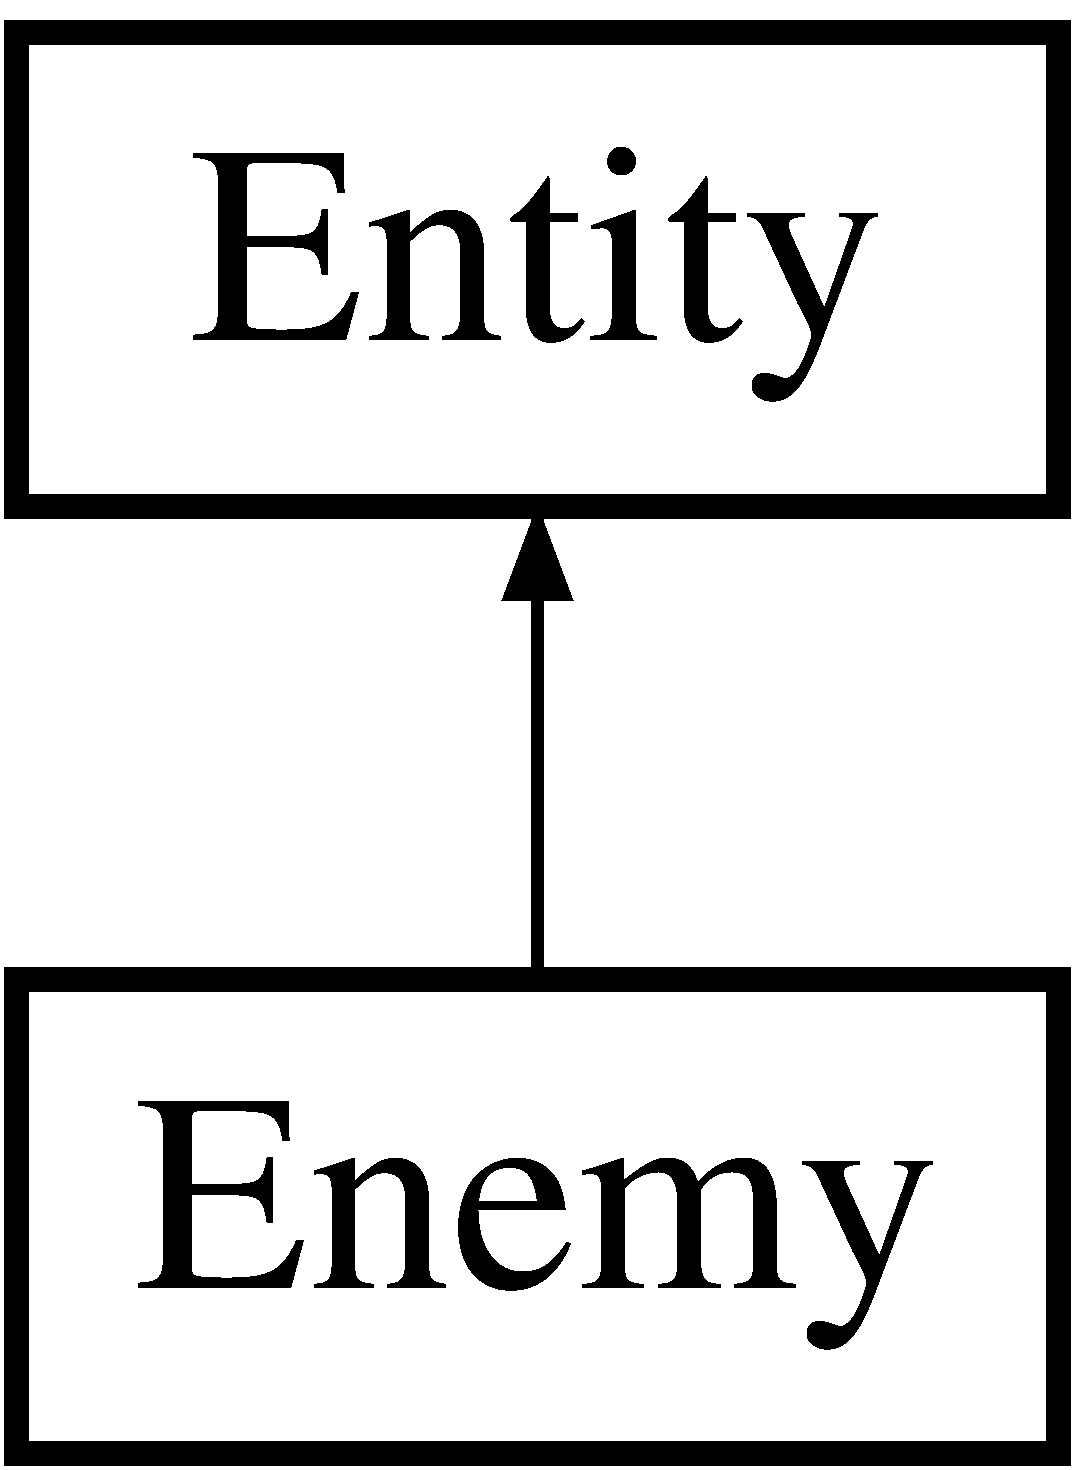
\includegraphics[height=2.000000cm]{class_enemy}
\end{center}
\end{figure}
\subsection*{Public Types}
\begin{DoxyCompactItemize}
\item 
enum {\bfseries Type} \{ {\bfseries F\-A\-S\-T}, 
{\bfseries N\-O\-R\-M\-A\-L}, 
{\bfseries P\-R\-E\-D\-I\-C\-T\-I\-O\-N}, 
{\bfseries R\-A\-N\-D\-O\-M}
 \}
\end{DoxyCompactItemize}
\subsection*{Public Member Functions}
\begin{DoxyCompactItemize}
\item 
\hypertarget{class_enemy_a0bbb5db5819fcfa1d83f222f38f96c24}{{\bfseries Enemy} (Type type, \hyperlink{class_scenario}{Scenario} $\ast$scenario)}\label{class_enemy_a0bbb5db5819fcfa1d83f222f38f96c24}

\item 
\hypertarget{class_enemy_ad55ee71b5a8c23fbd00b3c368b90cc64}{void {\bfseries update} ()}\label{class_enemy_ad55ee71b5a8c23fbd00b3c368b90cc64}

\item 
bool \hyperlink{class_enemy_a2cce7194016cb90b9e457b3da131fd8a}{is\-Alive} ()
\item 
bool \hyperlink{class_enemy_aaab62fdc7c1ddcc63aca532bed8bf613}{is\-Vulnerable} ()
\item 
\hypertarget{class_enemy_ab45669434f4b9c028c9efde8fbeb27b7}{\hyperlink{class_vector2_d}{Vector2\-D} {\bfseries position\-Centered} ()}\label{class_enemy_ab45669434f4b9c028c9efde8fbeb27b7}

\item 
void \hyperlink{class_enemy_a8d18ac9c202950499f631169e8346c58}{record\-Player\-Position} (\hyperlink{class_vector2_d}{Vector2\-D} pos)
\begin{DoxyCompactList}\small\item\em Guarda la posición del jugador en la lista. \end{DoxyCompactList}\item 
\hypertarget{class_enemy_ab8bd4193b6250a1327d1bf9edc159ded}{\hyperlink{class_vector2_d}{Vector2\-D} {\bfseries destination\-Cell} ()}\label{class_enemy_ab8bd4193b6250a1327d1bf9edc159ded}

\end{DoxyCompactItemize}
\subsection*{Additional Inherited Members}


\subsection{Member Function Documentation}
\hypertarget{class_enemy_a2cce7194016cb90b9e457b3da131fd8a}{\index{Enemy@{Enemy}!is\-Alive@{is\-Alive}}
\index{is\-Alive@{is\-Alive}!Enemy@{Enemy}}
\subsubsection[{is\-Alive}]{\setlength{\rightskip}{0pt plus 5cm}bool Enemy\-::is\-Alive (
\begin{DoxyParamCaption}
{}
\end{DoxyParamCaption}
)}}\label{class_enemy_a2cce7194016cb90b9e457b3da131fd8a}
\begin{DoxyReturn}{Returns}

\end{DoxyReturn}
\hypertarget{class_enemy_aaab62fdc7c1ddcc63aca532bed8bf613}{\index{Enemy@{Enemy}!is\-Vulnerable@{is\-Vulnerable}}
\index{is\-Vulnerable@{is\-Vulnerable}!Enemy@{Enemy}}
\subsubsection[{is\-Vulnerable}]{\setlength{\rightskip}{0pt plus 5cm}bool Enemy\-::is\-Vulnerable (
\begin{DoxyParamCaption}
{}
\end{DoxyParamCaption}
)}}\label{class_enemy_aaab62fdc7c1ddcc63aca532bed8bf613}
\begin{DoxyReturn}{Returns}

\end{DoxyReturn}
\hypertarget{class_enemy_a8d18ac9c202950499f631169e8346c58}{\index{Enemy@{Enemy}!record\-Player\-Position@{record\-Player\-Position}}
\index{record\-Player\-Position@{record\-Player\-Position}!Enemy@{Enemy}}
\subsubsection[{record\-Player\-Position}]{\setlength{\rightskip}{0pt plus 5cm}void Enemy\-::record\-Player\-Position (
\begin{DoxyParamCaption}
\item[{{\bf Vector2\-D}}]{pos}
\end{DoxyParamCaption}
)}}\label{class_enemy_a8d18ac9c202950499f631169e8346c58}


Guarda la posición del jugador en la lista. 


\begin{DoxyParams}{Parameters}
{\em pos} & posición del jugador \\
\hline
\end{DoxyParams}


The documentation for this class was generated from the following files\-:\begin{DoxyCompactItemize}
\item 
Multicoco\-S\-D\-L/\-Multicoco\-S\-D\-L/enemy.\-h\item 
Multicoco\-S\-D\-L/\-Multicoco\-S\-D\-L/enemy.\-cpp\end{DoxyCompactItemize}

\hypertarget{class_entity}{\section{Entity Class Reference}
\label{class_entity}\index{Entity@{Entity}}
}


{\ttfamily \#include $<$entity.\-h$>$}

Inheritance diagram for Entity\-:\begin{figure}[H]
\begin{center}
\leavevmode
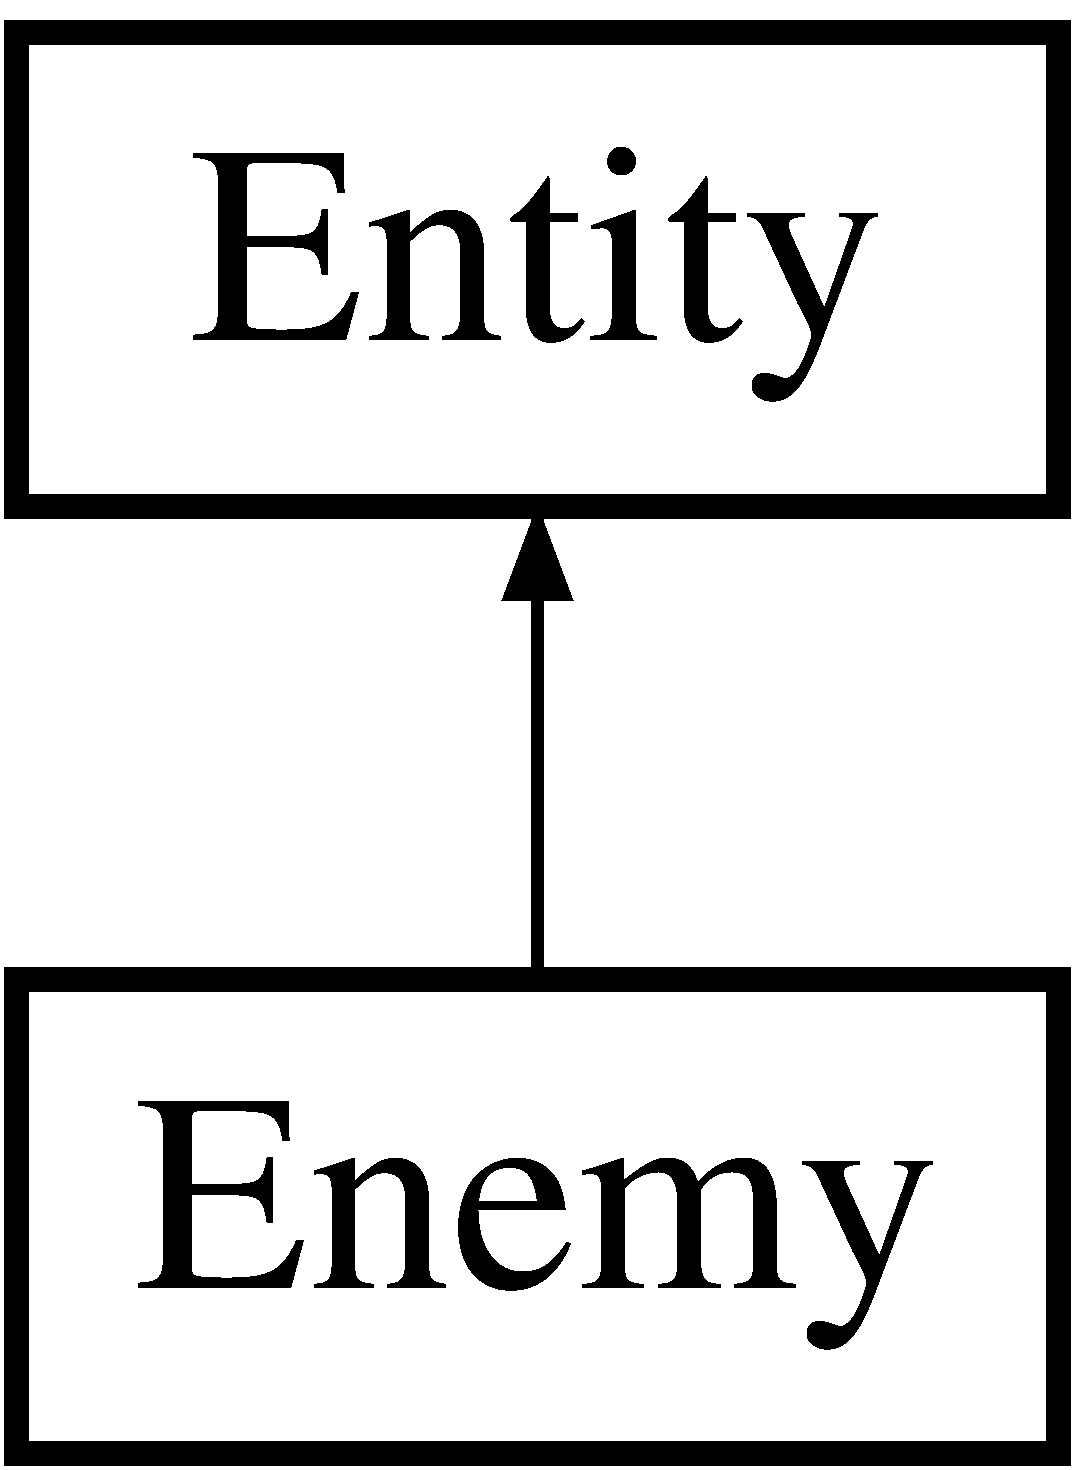
\includegraphics[height=2.000000cm]{class_entity}
\end{center}
\end{figure}
\subsection*{Public Member Functions}
\begin{DoxyCompactItemize}
\item 
\hypertarget{class_entity_a93306ecdce9446da37560f5f2b5307c0}{void {\bfseries set\-Position} (float x, float y)}\label{class_entity_a93306ecdce9446da37560f5f2b5307c0}

\item 
\hypertarget{class_entity_a4a3db66e94bc72170bcda8b12c8459e5}{void {\bfseries set\-Position} (\hyperlink{class_vector2_d}{Vector2\-D} v)}\label{class_entity_a4a3db66e94bc72170bcda8b12c8459e5}

\item 
\hypertarget{class_entity_a9e3c0cf949f611403d3166554a47031d}{void {\bfseries set\-Direction} (float x, float y)}\label{class_entity_a9e3c0cf949f611403d3166554a47031d}

\item 
\hypertarget{class_entity_a881f23d8c1d5eed41935540af9a84222}{void {\bfseries set\-Direction} (\hyperlink{class_vector2_d}{Vector2\-D} \&v)}\label{class_entity_a881f23d8c1d5eed41935540af9a84222}

\item 
\hypertarget{class_entity_a10c4181924679903a918174e7772abf9}{void {\bfseries set\-Visible} (bool v)}\label{class_entity_a10c4181924679903a918174e7772abf9}

\item 
\hypertarget{class_entity_af0dc11f1a253b5c7c1bb07e76f8bc261}{void {\bfseries set\-Moving} (bool m)}\label{class_entity_af0dc11f1a253b5c7c1bb07e76f8bc261}

\item 
\hypertarget{class_entity_ae405331a64288b8fb4bfe05c66d58ace}{void {\bfseries set\-Sprite\-Sheet} (const char $\ast$file, int w, int h, int $\ast$animations, int n\-Animations)}\label{class_entity_ae405331a64288b8fb4bfe05c66d58ace}

\item 
\hypertarget{class_entity_ae83091bf9d06a5257cf3f571470383e5}{\hyperlink{class_sprite_sheet}{Sprite\-Sheet} \& {\bfseries sprite\-Sheet} ()}\label{class_entity_ae83091bf9d06a5257cf3f571470383e5}

\item 
\hypertarget{class_entity_a9f0c2c230382d8f4f19f6da86beb6384}{\hyperlink{class_collision_box}{Collision\-Box} \& {\bfseries collision\-Box} ()}\label{class_entity_a9f0c2c230382d8f4f19f6da86beb6384}

\item 
\hypertarget{class_entity_ad1e7b83b2f35e78e84b1705937309fe9}{void {\bfseries set\-Animation} (const char $\ast$name)}\label{class_entity_ad1e7b83b2f35e78e84b1705937309fe9}

\item 
\hypertarget{class_entity_a098d827982916bd7b3d13f6858c520d7}{bool {\bfseries is\-Visible} ()}\label{class_entity_a098d827982916bd7b3d13f6858c520d7}

\item 
\hypertarget{class_entity_aa208f77af13f749357d0151fdb5f8b34}{bool {\bfseries is\-Moving} ()}\label{class_entity_aa208f77af13f749357d0151fdb5f8b34}

\item 
\hypertarget{class_entity_a1183593ad58f48225058ba545880e834}{\hyperlink{class_vector2_d}{Vector2\-D} \& {\bfseries position} ()}\label{class_entity_a1183593ad58f48225058ba545880e834}

\item 
\hypertarget{class_entity_a4d0d62c67cdf86694c45333608922eb0}{\hyperlink{class_vector2_d}{Vector2\-D} \& {\bfseries direction} ()}\label{class_entity_a4d0d62c67cdf86694c45333608922eb0}

\item 
\hypertarget{class_entity_aed73e98b980b85833428c935cc1c69f8}{virtual void {\bfseries update} ()}\label{class_entity_aed73e98b980b85833428c935cc1c69f8}

\item 
\hypertarget{class_entity_ac1f12a5f7922624ee7ced15be3b884de}{void {\bfseries move} ()}\label{class_entity_ac1f12a5f7922624ee7ced15be3b884de}

\item 
\hypertarget{class_entity_a2fc98106ec767b2d2a6fbd9377f8750f}{void {\bfseries move\-To\-Previous\-Position} ()}\label{class_entity_a2fc98106ec767b2d2a6fbd9377f8750f}

\item 
\hypertarget{class_entity_a7fef3cd0e1983019e27047d2cceb0f1d}{void {\bfseries render} (S\-D\-L\-\_\-\-Surface $\ast$screen, bool show\-Debug\-Graphics=false)}\label{class_entity_a7fef3cd0e1983019e27047d2cceb0f1d}

\end{DoxyCompactItemize}
\subsection*{Protected Attributes}
\begin{DoxyCompactItemize}
\item 
\hypertarget{class_entity_a032fc6b59ce0125aaa590ba45a0e160b}{\hyperlink{class_vector2_d}{Vector2\-D} {\bfseries \-\_\-position}}\label{class_entity_a032fc6b59ce0125aaa590ba45a0e160b}

\item 
\hypertarget{class_entity_ad4c3e1eec02d5d7417a22e6f759fa249}{\hyperlink{class_vector2_d}{Vector2\-D} {\bfseries \-\_\-previous\-Position}}\label{class_entity_ad4c3e1eec02d5d7417a22e6f759fa249}

\item 
\hypertarget{class_entity_a87e3e972e084ed0900466e47fd1c8d99}{\hyperlink{class_vector2_d}{Vector2\-D} {\bfseries \-\_\-direction}}\label{class_entity_a87e3e972e084ed0900466e47fd1c8d99}

\item 
\hypertarget{class_entity_ae227fafdb344eb23c136552b1c57910c}{bool {\bfseries \-\_\-visible}}\label{class_entity_ae227fafdb344eb23c136552b1c57910c}

\item 
\hypertarget{class_entity_a2a1cfc1dc1c719eb49a9b7aa3922b981}{bool {\bfseries \-\_\-moving}}\label{class_entity_a2a1cfc1dc1c719eb49a9b7aa3922b981}

\item 
\hypertarget{class_entity_ac27b197182854d0af144dcbbc54d7151}{\hyperlink{class_sprite_sheet}{Sprite\-Sheet} $\ast$ {\bfseries \-\_\-sprite}}\label{class_entity_ac27b197182854d0af144dcbbc54d7151}

\item 
\hypertarget{class_entity_ad83773979b654d923fca4b83f805368d}{\hyperlink{class_collision_box}{Collision\-Box} $\ast$ {\bfseries \-\_\-collision\-Box}}\label{class_entity_ad83773979b654d923fca4b83f805368d}

\end{DoxyCompactItemize}


\subsection{Detailed Description}
Representa cualquier objeto que se muestra en el juego, desde Pacman a las monedas. 

The documentation for this class was generated from the following file\-:\begin{DoxyCompactItemize}
\item 
Multicoco\-S\-D\-L/\-Multicoco\-S\-D\-L/entity.\-h\end{DoxyCompactItemize}

\hypertarget{class_music}{\section{Music Class Reference}
\label{class_music}\index{Music@{Music}}
}
\subsection*{Public Member Functions}
\begin{DoxyCompactItemize}
\item 
\hypertarget{class_music_a85decb61f24531a66bf3943945f3f40a}{{\bfseries Music} (const char $\ast$file)}\label{class_music_a85decb61f24531a66bf3943945f3f40a}

\item 
\hypertarget{class_music_a54b941f6f7634d7f99b473c78fe6e4da}{void {\bfseries play} ()}\label{class_music_a54b941f6f7634d7f99b473c78fe6e4da}

\item 
\hypertarget{class_music_a1cd9e6b64bfcaa6c75cfb62d1ddfe9b6}{void {\bfseries play\-Loop} ()}\label{class_music_a1cd9e6b64bfcaa6c75cfb62d1ddfe9b6}

\item 
\hypertarget{class_music_a008211b514c1c89c15399d3384d3fcea}{void {\bfseries stop} ()}\label{class_music_a008211b514c1c89c15399d3384d3fcea}

\end{DoxyCompactItemize}


The documentation for this class was generated from the following files\-:\begin{DoxyCompactItemize}
\item 
Multicoco\-S\-D\-L/\-Multicoco\-S\-D\-L/music.\-h\item 
Multicoco\-S\-D\-L/\-Multicoco\-S\-D\-L/music.\-cpp\end{DoxyCompactItemize}

\hypertarget{category_n_s_application_07_s_d_l___missing___methods_08}{\section{N\-S\-Application(S\-D\-L\-\_\-\-Missing\-\_\-\-Methods) Category Reference}
\label{category_n_s_application_07_s_d_l___missing___methods_08}\index{N\-S\-Application(\-S\-D\-L\-\_\-\-Missing\-\_\-\-Methods)@{N\-S\-Application(\-S\-D\-L\-\_\-\-Missing\-\_\-\-Methods)}}
}
\subsection*{Instance Methods}
\begin{DoxyCompactItemize}
\item 
\hypertarget{category_n_s_application_07_s_d_l___missing___methods_08_abc77a503ce35ae00353bc65f8d3f3f3e}{(void) -\/ {\bfseries set\-Apple\-Menu\-:}}\label{category_n_s_application_07_s_d_l___missing___methods_08_abc77a503ce35ae00353bc65f8d3f3f3e}

\end{DoxyCompactItemize}


The documentation for this category was generated from the following file\-:\begin{DoxyCompactItemize}
\item 
Multicoco\-S\-D\-L/\-Multicoco\-S\-D\-L/S\-D\-L\-Main.\-m\end{DoxyCompactItemize}

\hypertarget{category_n_s_application_07_s_d_l_application_08}{\section{N\-S\-Application(S\-D\-L\-Application) Category Reference}
\label{category_n_s_application_07_s_d_l_application_08}\index{N\-S\-Application(\-S\-D\-L\-Application)@{N\-S\-Application(\-S\-D\-L\-Application)}}
}


The documentation for this category was generated from the following file\-:\begin{DoxyCompactItemize}
\item 
Multicoco\-S\-D\-L/\-Multicoco\-S\-D\-L/S\-D\-L\-Main.\-m\end{DoxyCompactItemize}

\hypertarget{category_n_s_string_07_replace_sub_string_08}{\section{N\-S\-String(Replace\-Sub\-String) Category Reference}
\label{category_n_s_string_07_replace_sub_string_08}\index{N\-S\-String(\-Replace\-Sub\-String)@{N\-S\-String(\-Replace\-Sub\-String)}}
}


The documentation for this category was generated from the following file\-:\begin{DoxyCompactItemize}
\item 
Multicoco\-S\-D\-L/\-Multicoco\-S\-D\-L/S\-D\-L\-Main.\-m\end{DoxyCompactItemize}

\hypertarget{class_scenario}{\section{Scenario Class Reference}
\label{class_scenario}\index{Scenario@{Scenario}}
}
\subsection*{Public Member Functions}
\begin{DoxyCompactItemize}
\item 
\hyperlink{class_scenario_a8189517ddf6e34f006df80cf8fb6a71f}{Scenario} (unsigned int h\-Size, unsigned int v\-Size, \hyperlink{class_vector2_d}{Vector2\-D} position)
\begin{DoxyCompactList}\small\item\em Crea un escenario de forma aleatoria, excepto el cuadro central que sirve como casa para los enemigos. \end{DoxyCompactList}\item 
\hypertarget{class_scenario_ad4e825abd3b69f660fe0eadf02496321}{{\bfseries Scenario} (const char $\ast$file)}\label{class_scenario_ad4e825abd3b69f660fe0eadf02496321}

\item 
\hypertarget{class_scenario_aa7e7548858cbc52614d46723c0333038}{\hyperlink{class_scenario_aa7e7548858cbc52614d46723c0333038}{$\sim$\-Scenario} ()}\label{class_scenario_aa7e7548858cbc52614d46723c0333038}

\begin{DoxyCompactList}\small\item\em Destructor. Libera los recursos. \end{DoxyCompactList}\item 
unsigned int \hyperlink{class_scenario_a457b1626f68e6a2659aaf6a2038c7aa1}{horizontal\-Size} ()
\begin{DoxyCompactList}\small\item\em Numero de casillas en horizontal del escenario. \end{DoxyCompactList}\item 
unsigned int \hyperlink{class_scenario_a210693b48fbbc4b02ebc4824131ea0ad}{vertical\-Size} ()
\begin{DoxyCompactList}\small\item\em Numero de casillas en vertical. \end{DoxyCompactList}\item 
unsigned int \hyperlink{class_scenario_a2b098ae8cf7bfdbf9d281d72e241bb88}{width} ()
\begin{DoxyCompactList}\small\item\em Ancho total del escenario en pixeles. \end{DoxyCompactList}\item 
unsigned int \hyperlink{class_scenario_ad46654c66f78b69b2ceff9fbed9fd31d}{height} ()
\begin{DoxyCompactList}\small\item\em Altura total del escenario en pixeles. \end{DoxyCompactList}\item 
\hypertarget{class_scenario_a5c42393e886cffc17d929d518dfec392}{\hyperlink{class_vector2_d}{Vector2\-D} {\bfseries enemy\-Spawning\-Cell} ()}\label{class_scenario_a5c42393e886cffc17d929d518dfec392}

\item 
\hyperlink{class_vector2_d}{Vector2\-D} \hyperlink{class_scenario_a867a2986faf6ab2b027d783edc0d9a00}{player\-Spawning\-Cell} ()
\begin{DoxyCompactList}\small\item\em Casilla donde aparece el jugador. \end{DoxyCompactList}\item 
\hyperlink{class_sprite_sheet}{Sprite\-Sheet} \& \hyperlink{class_scenario_a823adba186e44615fcb34990713d9d4c}{sprite\-Sheet} ()
\begin{DoxyCompactList}\small\item\em Acceso al sprite asociado. \end{DoxyCompactList}\item 
\hyperlink{class_vector2_d}{Vector2\-D} \hyperlink{class_scenario_a95e4e91a8989095a0aff9eccdc4b2180}{player\-Spawning\-Position} ()
\begin{DoxyCompactList}\small\item\em Posicion donde aparece el jugador. \end{DoxyCompactList}\item 
\hyperlink{class_vector2_d}{Vector2\-D} \hyperlink{class_scenario_a2415ebf67ac30ed8a32f074a07b16904}{enemy\-Spawning\-Position} ()
\begin{DoxyCompactList}\small\item\em Posicion donde aparecen los enemigos. \end{DoxyCompactList}\item 
\hypertarget{class_scenario_a6b4df480c24ac6e608b0db70213d1756}{void {\bfseries set\-Enemy\-Spawning\-Cell} (unsigned int x, unsigned int y)}\label{class_scenario_a6b4df480c24ac6e608b0db70213d1756}

\item 
\hypertarget{class_scenario_a696289efceb56b7e53b9ebd657b69c3e}{void {\bfseries set\-Player\-Spawning\-Cell} (unsigned int x, unsigned int y)}\label{class_scenario_a696289efceb56b7e53b9ebd657b69c3e}

\item 
\hypertarget{class_scenario_a75e4afed8ae12a12fbf822d2a23aebf4}{void \hyperlink{class_scenario_a75e4afed8ae12a12fbf822d2a23aebf4}{set\-Random\-Player\-Spawning\-Cell} ()}\label{class_scenario_a75e4afed8ae12a12fbf822d2a23aebf4}

\begin{DoxyCompactList}\small\item\em Asigna una celda aleatoria donde aparecerá el jugador. \end{DoxyCompactList}\item 
\hypertarget{class_scenario_a3d9f5b2d8f7fe2ff636c4d9d7b96caa7}{void {\bfseries set\-Sprite\-Sheet} (const char $\ast$file, int w, int h, int $\ast$animations, int n\-Animations)}\label{class_scenario_a3d9f5b2d8f7fe2ff636c4d9d7b96caa7}

\item 
void \hyperlink{class_scenario_a264bcbcfb4cf26c79fcd0bb92e6a6991}{set\-Wall\-Sprite} (unsigned int pos)
\begin{DoxyCompactList}\small\item\em Indica qué fila de la plantilla asignada corresponde al sprite del muro. \end{DoxyCompactList}\item 
void \hyperlink{class_scenario_a5a16a90c0b3bbccc8b79316a159631ec}{set\-Corridor\-Sprite} (unsigned int pos)
\begin{DoxyCompactList}\small\item\em Indica qué fila de la plantilla asignada corresponde al sprite del pasillo. \end{DoxyCompactList}\item 
\hypertarget{class_scenario_abc3b44c28bf74a91f9e7a052f8010269}{bool {\bfseries save} (const char $\ast$file)}\label{class_scenario_abc3b44c28bf74a91f9e7a052f8010269}

\item 
bool \hyperlink{class_scenario_ab0df7d43602535a535b30db82115c912}{is\-Wall} (int x, int y)
\begin{DoxyCompactList}\small\item\em Indica si la casilla es una pared. \end{DoxyCompactList}\item 
bool \hyperlink{class_scenario_ac55d32b9280231f5f3c608b88fb79222}{is\-Corridor} (int x, int y)
\begin{DoxyCompactList}\small\item\em Indica si la casilla es un pasillo. \end{DoxyCompactList}\item 
\hyperlink{class_vector2_d}{Vector2\-D} \hyperlink{class_scenario_ad48f84e44fef3ae985cdd3245acf065d}{cell} (int x, int y)
\begin{DoxyCompactList}\small\item\em Calcula que casilla del escenario corresponde con dichas coordenadas. \end{DoxyCompactList}\item 
\hyperlink{class_vector2_d}{Vector2\-D} \hyperlink{class_scenario_a7164ece5fdfe79405863ebed3590fb0d}{cell} (\hyperlink{class_vector2_d}{Vector2\-D} pos)
\begin{DoxyCompactList}\small\item\em Calcula que casilla del escenario corresponde con dichas coordenadas. \end{DoxyCompactList}\item 
\hypertarget{class_scenario_a3a0f6033d2652feb47b69d9838af31b0}{\hyperlink{class_vector2_d}{Vector2\-D} \hyperlink{class_scenario_a3a0f6033d2652feb47b69d9838af31b0}{cell\-Position} (unsigned int x, unsigned int y)}\label{class_scenario_a3a0f6033d2652feb47b69d9838af31b0}

\begin{DoxyCompactList}\small\item\em Posicion en pixeles de una celda cada. \end{DoxyCompactList}\item 
std\-::vector$<$ \hyperlink{class_vector2_d}{Vector2\-D} $>$ \hyperlink{class_scenario_a501950a0beb5aaeb0e31704818097ae4}{avalible\-Directions} (int pos\-X, int pos\-Y)
\begin{DoxyCompactList}\small\item\em Direcciones en las que se puede ir sin colisionar con una pared. \end{DoxyCompactList}\item 
bool \hyperlink{class_scenario_a4cad7d000c20baab4301e2561c82f514}{collides} (\hyperlink{class_entity}{Entity} \&object)
\begin{DoxyCompactList}\small\item\em Comprueba si un objeto pasado colisiona con alguna de las paredes. \end{DoxyCompactList}\item 
\hypertarget{class_scenario_a0789f28647f405ff79bde8a2cb03931c}{std\-::list$<$ \hyperlink{class_vector2_d}{Vector2\-D} $>$ \hyperlink{class_scenario_a0789f28647f405ff79bde8a2cb03931c}{corridor\-Cells} ()}\label{class_scenario_a0789f28647f405ff79bde8a2cb03931c}

\begin{DoxyCompactList}\small\item\em Lista de celdas del escenario que no son pared. \end{DoxyCompactList}\item 
std\-::list$<$ \hyperlink{class_vector2_d}{Vector2\-D} $>$ \hyperlink{class_scenario_af50bc8b0ac052db72a77a1d265078b6b}{corridor\-Positions} ()
\begin{DoxyCompactList}\small\item\em Posiciones en pixels de todas las casillas que son pasillos. \end{DoxyCompactList}\item 
std\-::list$<$ \hyperlink{class_vector2_d}{Vector2\-D} $>$ \hyperlink{class_scenario_abf51342b7ef5c8461b05085a085af2b2}{corridor\-Positions\-Without\-Ghost\-House} ()
\begin{DoxyCompactList}\small\item\em Posiciones en pixels de todas las casillas que son pasillos sin tener en cuenta la casa de los fantasmas. \end{DoxyCompactList}\item 
void \hyperlink{class_scenario_aa1479dc291201e8d2e3cbad06f87659b}{render} (S\-D\-L\-\_\-\-Surface $\ast$screen, bool show\-Debug\-Graphics=false)
\begin{DoxyCompactList}\small\item\em Dibuja el escenario en la pantalla en la posicion indicada. \end{DoxyCompactList}\end{DoxyCompactItemize}


\subsection{Constructor \& Destructor Documentation}
\hypertarget{class_scenario_a8189517ddf6e34f006df80cf8fb6a71f}{\index{Scenario@{Scenario}!Scenario@{Scenario}}
\index{Scenario@{Scenario}!Scenario@{Scenario}}
\subsubsection[{Scenario}]{\setlength{\rightskip}{0pt plus 5cm}Scenario\-::\-Scenario (
\begin{DoxyParamCaption}
\item[{unsigned int}]{h\-Size, }
\item[{unsigned int}]{v\-Size, }
\item[{{\bf Vector2\-D}}]{position}
\end{DoxyParamCaption}
)}}\label{class_scenario_a8189517ddf6e34f006df80cf8fb6a71f}


Crea un escenario de forma aleatoria, excepto el cuadro central que sirve como casa para los enemigos. 


\begin{DoxyParams}{Parameters}
{\em h\-Size} & Tamaño horizontal del tablero en número de casillas. \\
\hline
{\em v\-Size} & Tamaño vertical del tablero en número de casillas. \\
\hline
{\em position} & Posicion en la pantalla del punto central del laberinto. \\
\hline
\end{DoxyParams}


\subsection{Member Function Documentation}
\hypertarget{class_scenario_a501950a0beb5aaeb0e31704818097ae4}{\index{Scenario@{Scenario}!avalible\-Directions@{avalible\-Directions}}
\index{avalible\-Directions@{avalible\-Directions}!Scenario@{Scenario}}
\subsubsection[{avalible\-Directions}]{\setlength{\rightskip}{0pt plus 5cm}std\-::vector$<$ {\bf Vector2\-D} $>$ Scenario\-::avalible\-Directions (
\begin{DoxyParamCaption}
\item[{int}]{pos\-X, }
\item[{int}]{pos\-Y}
\end{DoxyParamCaption}
)}}\label{class_scenario_a501950a0beb5aaeb0e31704818097ae4}


Direcciones en las que se puede ir sin colisionar con una pared. 


\begin{DoxyParams}{Parameters}
{\em pos\-X} & Coordenada X en pixels de la posicion. \\
\hline
{\em pos\-Y} & Coordenada Y en pixels de la posicion. \\
\hline
\end{DoxyParams}
\begin{DoxyReturn}{Returns}
Vector con las direcciones en las que se puede ir desde la actual sin colisionar con una pared. 
\end{DoxyReturn}
\hypertarget{class_scenario_ad48f84e44fef3ae985cdd3245acf065d}{\index{Scenario@{Scenario}!cell@{cell}}
\index{cell@{cell}!Scenario@{Scenario}}
\subsubsection[{cell}]{\setlength{\rightskip}{0pt plus 5cm}{\bf Vector2\-D} Scenario\-::cell (
\begin{DoxyParamCaption}
\item[{int}]{x, }
\item[{int}]{y}
\end{DoxyParamCaption}
)}}\label{class_scenario_ad48f84e44fef3ae985cdd3245acf065d}


Calcula que casilla del escenario corresponde con dichas coordenadas. 


\begin{DoxyParams}{Parameters}
{\em x} & Coordenada X. \\
\hline
{\em y} & Coordenada Y. \\
\hline
\end{DoxyParams}
\begin{DoxyReturn}{Returns}
Celda que corresponde a las coordenadas x e y. 
\end{DoxyReturn}
\hypertarget{class_scenario_a7164ece5fdfe79405863ebed3590fb0d}{\index{Scenario@{Scenario}!cell@{cell}}
\index{cell@{cell}!Scenario@{Scenario}}
\subsubsection[{cell}]{\setlength{\rightskip}{0pt plus 5cm}{\bf Vector2\-D} Scenario\-::cell (
\begin{DoxyParamCaption}
\item[{{\bf Vector2\-D}}]{pos}
\end{DoxyParamCaption}
)}}\label{class_scenario_a7164ece5fdfe79405863ebed3590fb0d}


Calcula que casilla del escenario corresponde con dichas coordenadas. 


\begin{DoxyParams}{Parameters}
{\em pos} & Posicion de la casilla. \\
\hline
\end{DoxyParams}
\begin{DoxyReturn}{Returns}
Celda que corresponde a las coordenadas x e y. 
\end{DoxyReturn}
\hypertarget{class_scenario_a4cad7d000c20baab4301e2561c82f514}{\index{Scenario@{Scenario}!collides@{collides}}
\index{collides@{collides}!Scenario@{Scenario}}
\subsubsection[{collides}]{\setlength{\rightskip}{0pt plus 5cm}bool Scenario\-::collides (
\begin{DoxyParamCaption}
\item[{{\bf Entity} \&}]{object}
\end{DoxyParamCaption}
)}}\label{class_scenario_a4cad7d000c20baab4301e2561c82f514}


Comprueba si un objeto pasado colisiona con alguna de las paredes. 


\begin{DoxyParams}{Parameters}
{\em object} & Objeto con el que comprobar la colisión. \\
\hline
\end{DoxyParams}
\begin{DoxyReturn}{Returns}
true si el objeto colisiona con alguna pared, false si no colisiona con ninguno. 
\end{DoxyReturn}
\hypertarget{class_scenario_af50bc8b0ac052db72a77a1d265078b6b}{\index{Scenario@{Scenario}!corridor\-Positions@{corridor\-Positions}}
\index{corridor\-Positions@{corridor\-Positions}!Scenario@{Scenario}}
\subsubsection[{corridor\-Positions}]{\setlength{\rightskip}{0pt plus 5cm}std\-::list$<$ {\bf Vector2\-D} $>$ Scenario\-::corridor\-Positions (
\begin{DoxyParamCaption}
{}
\end{DoxyParamCaption}
)}}\label{class_scenario_af50bc8b0ac052db72a77a1d265078b6b}


Posiciones en pixels de todas las casillas que son pasillos. 

\begin{DoxyReturn}{Returns}
Lista conteniendo las coordenadas de las casillas que son pasillo. 
\end{DoxyReturn}
\hypertarget{class_scenario_abf51342b7ef5c8461b05085a085af2b2}{\index{Scenario@{Scenario}!corridor\-Positions\-Without\-Ghost\-House@{corridor\-Positions\-Without\-Ghost\-House}}
\index{corridor\-Positions\-Without\-Ghost\-House@{corridor\-Positions\-Without\-Ghost\-House}!Scenario@{Scenario}}
\subsubsection[{corridor\-Positions\-Without\-Ghost\-House}]{\setlength{\rightskip}{0pt plus 5cm}std\-::list$<$ {\bf Vector2\-D} $>$ Scenario\-::corridor\-Positions\-Without\-Ghost\-House (
\begin{DoxyParamCaption}
{}
\end{DoxyParamCaption}
)}}\label{class_scenario_abf51342b7ef5c8461b05085a085af2b2}


Posiciones en pixels de todas las casillas que son pasillos sin tener en cuenta la casa de los fantasmas. 

\begin{DoxyReturn}{Returns}
Lista conteniendo las coordenadas de las casillas que son pasillo. 
\end{DoxyReturn}
\hypertarget{class_scenario_a2415ebf67ac30ed8a32f074a07b16904}{\index{Scenario@{Scenario}!enemy\-Spawning\-Position@{enemy\-Spawning\-Position}}
\index{enemy\-Spawning\-Position@{enemy\-Spawning\-Position}!Scenario@{Scenario}}
\subsubsection[{enemy\-Spawning\-Position}]{\setlength{\rightskip}{0pt plus 5cm}{\bf Vector2\-D} Scenario\-::enemy\-Spawning\-Position (
\begin{DoxyParamCaption}
{}
\end{DoxyParamCaption}
)}}\label{class_scenario_a2415ebf67ac30ed8a32f074a07b16904}


Posicion donde aparecen los enemigos. 

\begin{DoxyReturn}{Returns}
Vector con la posicion en pixeles donde aparecen los enemigos. 
\end{DoxyReturn}
\hypertarget{class_scenario_ad46654c66f78b69b2ceff9fbed9fd31d}{\index{Scenario@{Scenario}!height@{height}}
\index{height@{height}!Scenario@{Scenario}}
\subsubsection[{height}]{\setlength{\rightskip}{0pt plus 5cm}unsigned int Scenario\-::height (
\begin{DoxyParamCaption}
{}
\end{DoxyParamCaption}
)}}\label{class_scenario_ad46654c66f78b69b2ceff9fbed9fd31d}


Altura total del escenario en pixeles. 

\begin{DoxyReturn}{Returns}
Tamaño vertical en pixels. 
\end{DoxyReturn}
\hypertarget{class_scenario_a457b1626f68e6a2659aaf6a2038c7aa1}{\index{Scenario@{Scenario}!horizontal\-Size@{horizontal\-Size}}
\index{horizontal\-Size@{horizontal\-Size}!Scenario@{Scenario}}
\subsubsection[{horizontal\-Size}]{\setlength{\rightskip}{0pt plus 5cm}unsigned int Scenario\-::horizontal\-Size (
\begin{DoxyParamCaption}
{}
\end{DoxyParamCaption}
)}}\label{class_scenario_a457b1626f68e6a2659aaf6a2038c7aa1}


Numero de casillas en horizontal del escenario. 

\begin{DoxyReturn}{Returns}
Tamaño horizontal en casillas del esceario. 
\end{DoxyReturn}
\hypertarget{class_scenario_ac55d32b9280231f5f3c608b88fb79222}{\index{Scenario@{Scenario}!is\-Corridor@{is\-Corridor}}
\index{is\-Corridor@{is\-Corridor}!Scenario@{Scenario}}
\subsubsection[{is\-Corridor}]{\setlength{\rightskip}{0pt plus 5cm}bool Scenario\-::is\-Corridor (
\begin{DoxyParamCaption}
\item[{int}]{x, }
\item[{int}]{y}
\end{DoxyParamCaption}
)}}\label{class_scenario_ac55d32b9280231f5f3c608b88fb79222}


Indica si la casilla es un pasillo. 


\begin{DoxyParams}{Parameters}
{\em x} & Posicion X de la casilla. \\
\hline
{\em y} & Posicion Y de la casilla. \\
\hline
\end{DoxyParams}
\begin{DoxyReturn}{Returns}
true si la casilla es un pasillo, false si es una pared. 
\end{DoxyReturn}
\hypertarget{class_scenario_ab0df7d43602535a535b30db82115c912}{\index{Scenario@{Scenario}!is\-Wall@{is\-Wall}}
\index{is\-Wall@{is\-Wall}!Scenario@{Scenario}}
\subsubsection[{is\-Wall}]{\setlength{\rightskip}{0pt plus 5cm}bool Scenario\-::is\-Wall (
\begin{DoxyParamCaption}
\item[{int}]{x, }
\item[{int}]{y}
\end{DoxyParamCaption}
)}}\label{class_scenario_ab0df7d43602535a535b30db82115c912}


Indica si la casilla es una pared. 


\begin{DoxyParams}{Parameters}
{\em x} & Posicion X de la casilla. \\
\hline
{\em y} & Posicion Y de la casilla. \\
\hline
\end{DoxyParams}
\begin{DoxyReturn}{Returns}
true si la casilla es una pared, false si es un pasillo. 
\end{DoxyReturn}
\hypertarget{class_scenario_a867a2986faf6ab2b027d783edc0d9a00}{\index{Scenario@{Scenario}!player\-Spawning\-Cell@{player\-Spawning\-Cell}}
\index{player\-Spawning\-Cell@{player\-Spawning\-Cell}!Scenario@{Scenario}}
\subsubsection[{player\-Spawning\-Cell}]{\setlength{\rightskip}{0pt plus 5cm}{\bf Vector2\-D} Scenario\-::player\-Spawning\-Cell (
\begin{DoxyParamCaption}
{}
\end{DoxyParamCaption}
)}}\label{class_scenario_a867a2986faf6ab2b027d783edc0d9a00}


Casilla donde aparece el jugador. 

\begin{DoxyReturn}{Returns}
Vector con la posicion en casillas donde aparece el jugador. 
\end{DoxyReturn}
\hypertarget{class_scenario_a95e4e91a8989095a0aff9eccdc4b2180}{\index{Scenario@{Scenario}!player\-Spawning\-Position@{player\-Spawning\-Position}}
\index{player\-Spawning\-Position@{player\-Spawning\-Position}!Scenario@{Scenario}}
\subsubsection[{player\-Spawning\-Position}]{\setlength{\rightskip}{0pt plus 5cm}{\bf Vector2\-D} Scenario\-::player\-Spawning\-Position (
\begin{DoxyParamCaption}
{}
\end{DoxyParamCaption}
)}}\label{class_scenario_a95e4e91a8989095a0aff9eccdc4b2180}


Posicion donde aparece el jugador. 

\begin{DoxyReturn}{Returns}
Vector con la posicion en pixeles donde aparece el jugador. 
\end{DoxyReturn}
\hypertarget{class_scenario_aa1479dc291201e8d2e3cbad06f87659b}{\index{Scenario@{Scenario}!render@{render}}
\index{render@{render}!Scenario@{Scenario}}
\subsubsection[{render}]{\setlength{\rightskip}{0pt plus 5cm}void Scenario\-::render (
\begin{DoxyParamCaption}
\item[{S\-D\-L\-\_\-\-Surface $\ast$}]{screen, }
\item[{bool}]{show\-Debug\-Graphics = {\ttfamily false}}
\end{DoxyParamCaption}
)}}\label{class_scenario_aa1479dc291201e8d2e3cbad06f87659b}


Dibuja el escenario en la pantalla en la posicion indicada. 


\begin{DoxyParams}{Parameters}
{\em screen} & Pantalla en la que dibujar el escenario. \\
\hline
{\em position} & Punto central donde dibujar el laberinto. \\
\hline
\end{DoxyParams}
\begin{DoxyPrecond}{Precondition}
Se debe haber especificado la plantilla mediante set\-Sprite\-Sheet y vincular las imagenes de la pared y el pasillo mediante set\-Wall\-Sprite y set\-Corridor\-Sprite. 
\end{DoxyPrecond}
\hypertarget{class_scenario_a5a16a90c0b3bbccc8b79316a159631ec}{\index{Scenario@{Scenario}!set\-Corridor\-Sprite@{set\-Corridor\-Sprite}}
\index{set\-Corridor\-Sprite@{set\-Corridor\-Sprite}!Scenario@{Scenario}}
\subsubsection[{set\-Corridor\-Sprite}]{\setlength{\rightskip}{0pt plus 5cm}void Scenario\-::set\-Corridor\-Sprite (
\begin{DoxyParamCaption}
\item[{unsigned int}]{pos}
\end{DoxyParamCaption}
)}}\label{class_scenario_a5a16a90c0b3bbccc8b79316a159631ec}


Indica qué fila de la plantilla asignada corresponde al sprite del pasillo. 


\begin{DoxyParams}{Parameters}
{\em pos} & Posicion de la fila en la plantilla. \\
\hline
\end{DoxyParams}
\hypertarget{class_scenario_a264bcbcfb4cf26c79fcd0bb92e6a6991}{\index{Scenario@{Scenario}!set\-Wall\-Sprite@{set\-Wall\-Sprite}}
\index{set\-Wall\-Sprite@{set\-Wall\-Sprite}!Scenario@{Scenario}}
\subsubsection[{set\-Wall\-Sprite}]{\setlength{\rightskip}{0pt plus 5cm}void Scenario\-::set\-Wall\-Sprite (
\begin{DoxyParamCaption}
\item[{unsigned int}]{pos}
\end{DoxyParamCaption}
)}}\label{class_scenario_a264bcbcfb4cf26c79fcd0bb92e6a6991}


Indica qué fila de la plantilla asignada corresponde al sprite del muro. 


\begin{DoxyParams}{Parameters}
{\em pos} & Posicion de la fila en la plantilla. \\
\hline
\end{DoxyParams}
\hypertarget{class_scenario_a823adba186e44615fcb34990713d9d4c}{\index{Scenario@{Scenario}!sprite\-Sheet@{sprite\-Sheet}}
\index{sprite\-Sheet@{sprite\-Sheet}!Scenario@{Scenario}}
\subsubsection[{sprite\-Sheet}]{\setlength{\rightskip}{0pt plus 5cm}{\bf Sprite\-Sheet} \& Scenario\-::sprite\-Sheet (
\begin{DoxyParamCaption}
{}
\end{DoxyParamCaption}
)}}\label{class_scenario_a823adba186e44615fcb34990713d9d4c}


Acceso al sprite asociado. 

\begin{DoxyReturn}{Returns}
Referencia al sprite que usa el escenario para renderizarse. 
\end{DoxyReturn}
\hypertarget{class_scenario_a210693b48fbbc4b02ebc4824131ea0ad}{\index{Scenario@{Scenario}!vertical\-Size@{vertical\-Size}}
\index{vertical\-Size@{vertical\-Size}!Scenario@{Scenario}}
\subsubsection[{vertical\-Size}]{\setlength{\rightskip}{0pt plus 5cm}unsigned int Scenario\-::vertical\-Size (
\begin{DoxyParamCaption}
{}
\end{DoxyParamCaption}
)}}\label{class_scenario_a210693b48fbbc4b02ebc4824131ea0ad}


Numero de casillas en vertical. 

\begin{DoxyReturn}{Returns}
Tamaño vertical en casillas del escenario. 
\end{DoxyReturn}
\hypertarget{class_scenario_a2b098ae8cf7bfdbf9d281d72e241bb88}{\index{Scenario@{Scenario}!width@{width}}
\index{width@{width}!Scenario@{Scenario}}
\subsubsection[{width}]{\setlength{\rightskip}{0pt plus 5cm}unsigned int Scenario\-::width (
\begin{DoxyParamCaption}
{}
\end{DoxyParamCaption}
)}}\label{class_scenario_a2b098ae8cf7bfdbf9d281d72e241bb88}


Ancho total del escenario en pixeles. 

\begin{DoxyReturn}{Returns}
Tamaño horizontal en pixels. 
\end{DoxyReturn}


The documentation for this class was generated from the following files\-:\begin{DoxyCompactItemize}
\item 
Multicoco\-S\-D\-L/\-Multicoco\-S\-D\-L/scenario.\-h\item 
Multicoco\-S\-D\-L/\-Multicoco\-S\-D\-L/scenario.\-cpp\end{DoxyCompactItemize}

\hypertarget{interface_s_d_l_main}{\section{S\-D\-L\-Main Class Reference}
\label{interface_s_d_l_main}\index{S\-D\-L\-Main@{S\-D\-L\-Main}}
}
Inheritance diagram for S\-D\-L\-Main\-:\begin{figure}[H]
\begin{center}
\leavevmode
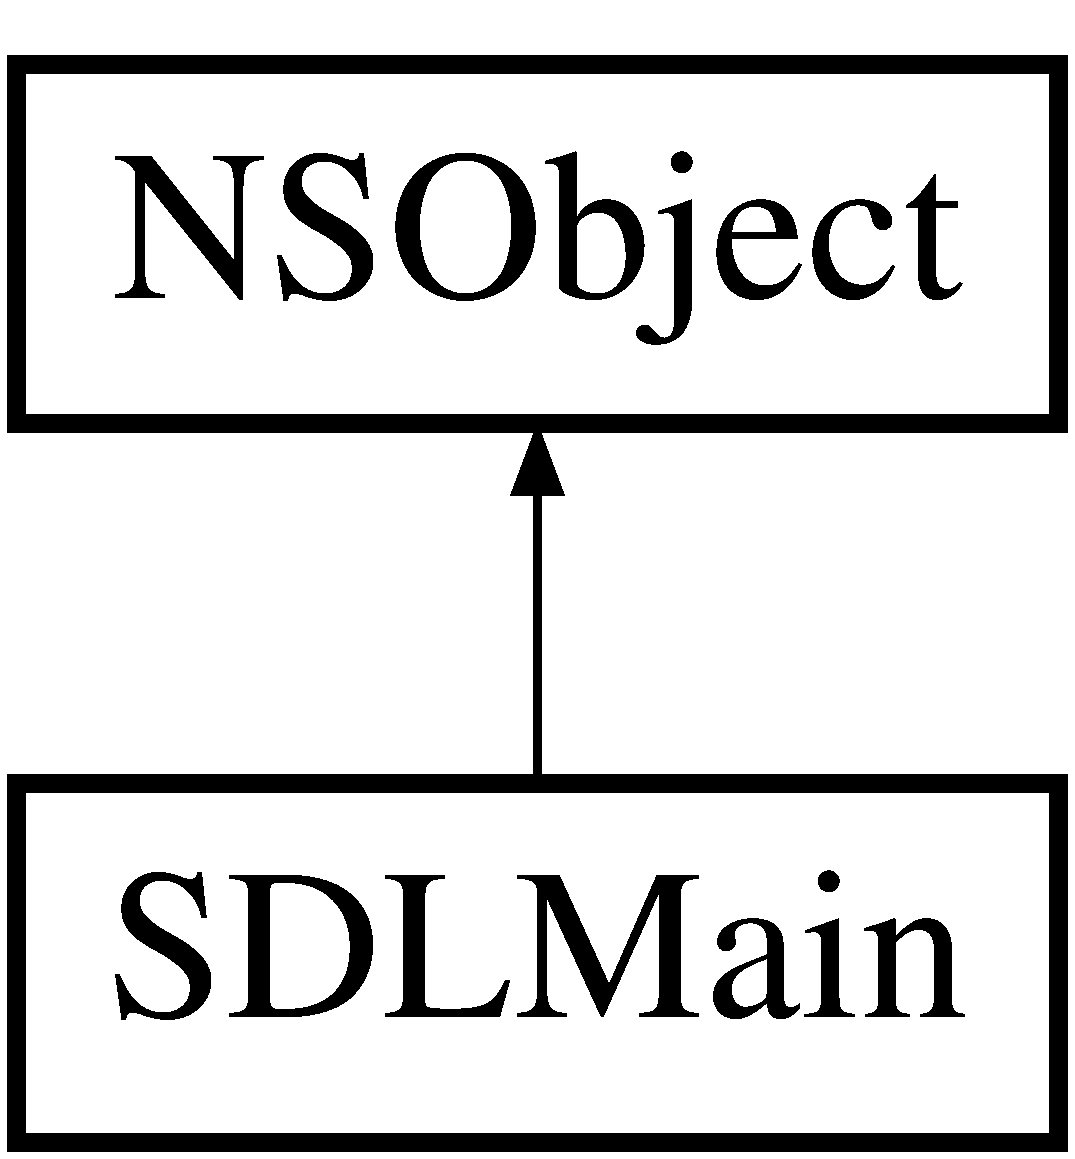
\includegraphics[height=2.000000cm]{interface_s_d_l_main}
\end{center}
\end{figure}


The documentation for this class was generated from the following file\-:\begin{DoxyCompactItemize}
\item 
Multicoco\-S\-D\-L/\-Multicoco\-S\-D\-L/S\-D\-L\-Main.\-h\end{DoxyCompactItemize}

\hypertarget{class_sound}{\section{Sound Class Reference}
\label{class_sound}\index{Sound@{Sound}}
}
\subsection*{Public Member Functions}
\begin{DoxyCompactItemize}
\item 
\hypertarget{class_sound_ae40758824408ca575a415dc99c4ff65f}{{\bfseries Sound} (const char $\ast$file)}\label{class_sound_ae40758824408ca575a415dc99c4ff65f}

\item 
\hypertarget{class_sound_a55b8e185d9c9014a26d36fdbc760993b}{bool {\bfseries play} ()}\label{class_sound_a55b8e185d9c9014a26d36fdbc760993b}

\item 
\hypertarget{class_sound_a167acf125385f6167eec534b9a164bf5}{bool {\bfseries play\-Loop} ()}\label{class_sound_a167acf125385f6167eec534b9a164bf5}

\item 
\hypertarget{class_sound_a3c393edeae934ea77f8af6b7c660614e}{bool {\bfseries is\-Playing} ()}\label{class_sound_a3c393edeae934ea77f8af6b7c660614e}

\item 
\hypertarget{class_sound_a07c551ab56d2f83a861a2f7fd81b480a}{void {\bfseries stop} ()}\label{class_sound_a07c551ab56d2f83a861a2f7fd81b480a}

\end{DoxyCompactItemize}


The documentation for this class was generated from the following files\-:\begin{DoxyCompactItemize}
\item 
Multicoco\-S\-D\-L/\-Multicoco\-S\-D\-L/sound.\-h\item 
Multicoco\-S\-D\-L/\-Multicoco\-S\-D\-L/sound.\-cpp\end{DoxyCompactItemize}

\hypertarget{class_sprite}{\section{Sprite Class Reference}
\label{class_sprite}\index{Sprite@{Sprite}}
}
\subsection*{Public Member Functions}
\begin{DoxyCompactItemize}
\item 
\hyperlink{class_sprite_a9c3c167ff294a793b862429798f3b17f}{Sprite} (S\-D\-L\-\_\-\-Surface $\ast$img, int animations, int w, int h)
\begin{DoxyCompactList}\small\item\em Construye un \hyperlink{class_sprite}{Sprite} animado a partir de una imagen con varios frames. \end{DoxyCompactList}\item 
\hypertarget{class_sprite_acbdf3175f0468de9d8451182c83ab4d3}{void {\bfseries render} (S\-D\-L\-\_\-\-Surface $\ast$screen, \hyperlink{class_vector2_d}{Vector2\-D} \&pos)}\label{class_sprite_acbdf3175f0468de9d8451182c83ab4d3}

\item 
\hypertarget{class_sprite_aad4221a926a6509c267dc309229fec6f}{void {\bfseries next\-Frame} ()}\label{class_sprite_aad4221a926a6509c267dc309229fec6f}

\item 
\hypertarget{class_sprite_ab5b585fd93678d8a6778e22dd24f1186}{void {\bfseries set\-Frame\-Skip} (unsigned int f)}\label{class_sprite_ab5b585fd93678d8a6778e22dd24f1186}

\end{DoxyCompactItemize}


\subsection{Constructor \& Destructor Documentation}
\hypertarget{class_sprite_a9c3c167ff294a793b862429798f3b17f}{\index{Sprite@{Sprite}!Sprite@{Sprite}}
\index{Sprite@{Sprite}!Sprite@{Sprite}}
\subsubsection[{Sprite}]{\setlength{\rightskip}{0pt plus 5cm}Sprite\-::\-Sprite (
\begin{DoxyParamCaption}
\item[{S\-D\-L\-\_\-\-Surface $\ast$}]{img, }
\item[{int}]{animations, }
\item[{int}]{w, }
\item[{int}]{h}
\end{DoxyParamCaption}
)}}\label{class_sprite_a9c3c167ff294a793b862429798f3b17f}


Construye un \hyperlink{class_sprite}{Sprite} animado a partir de una imagen con varios frames. 


\begin{DoxyParams}{Parameters}
{\em img} & \hyperlink{class_sprite}{Sprite} previamente cargado. Suele ser la fila de un \hyperlink{class_sprite_sheet}{Sprite\-Sheet}. \\
\hline
{\em animations} & Numero de frames de la animacion. \\
\hline
{\em w} & Ancho de cada frame del sprite. \\
\hline
{\em h} & Altura de cada frame del sprite. \\
\hline
\end{DoxyParams}


The documentation for this class was generated from the following files\-:\begin{DoxyCompactItemize}
\item 
Multicoco\-S\-D\-L/\-Multicoco\-S\-D\-L/sprite.\-h\item 
Multicoco\-S\-D\-L/\-Multicoco\-S\-D\-L/sprite.\-cpp\end{DoxyCompactItemize}

\hypertarget{class_sprite_sheet}{\section{Sprite\-Sheet Class Reference}
\label{class_sprite_sheet}\index{Sprite\-Sheet@{Sprite\-Sheet}}
}
\subsection*{Public Member Functions}
\begin{DoxyCompactItemize}
\item 
\hyperlink{class_sprite_sheet_a7271cbaa0719a4d5675ee8e94f85aa56}{Sprite\-Sheet} (const char $\ast$img, int w, int h, int $\ast$animations, int n\-Animations)
\begin{DoxyCompactList}\small\item\em Constructor de la plantilla de sprites. \end{DoxyCompactList}\item 
\hypertarget{class_sprite_sheet_a54a4dee6f85eb69fa699477764377d70}{unsigned int \hyperlink{class_sprite_sheet_a54a4dee6f85eb69fa699477764377d70}{sprite\-Width} ()}\label{class_sprite_sheet_a54a4dee6f85eb69fa699477764377d70}

\begin{DoxyCompactList}\small\item\em Ancho de cada frame individual del sprite. \end{DoxyCompactList}\item 
\hypertarget{class_sprite_sheet_add41556b6575aa5ad6a4fedfa9b8e5d6}{unsigned int \hyperlink{class_sprite_sheet_add41556b6575aa5ad6a4fedfa9b8e5d6}{sprite\-Height} ()}\label{class_sprite_sheet_add41556b6575aa5ad6a4fedfa9b8e5d6}

\begin{DoxyCompactList}\small\item\em Alto de cada frame individual del sprite. \end{DoxyCompactList}\item 
void \hyperlink{class_sprite_sheet_a807184db56f47aca2d7a603fd82604b5}{bind\-Animation} (unsigned int pos, const char $\ast$name)
\begin{DoxyCompactList}\small\item\em Vincula un nombre de animacion con una fila de la plantilla de animaciones. De esta forma es mas sencillo trabajar con distintas animaciones sin tener que saber el orden en que se encuentran en la plantilla. Por ejemplo, la animacion de moverse hacia la derecha esta en la primera fila de la plantilla, por lo que podemos vincular la posicion 0 de la plantilla con el nombre de animacion 'R\-I\-G\-H\-T' mediante blin\-Animation(0,\char`\"{}\-R\-I\-G\-H\-T\char`\"{}). De esta forma nos podremos referir a dicha animacion mas adelante mediante el nombre \char`\"{}\-R\-I\-G\-H\-T\char`\"{}. \end{DoxyCompactList}\item 
void \hyperlink{class_sprite_sheet_aa4279b765a0c354cd748b522755ca540}{set\-Animation} (const std\-::string name)
\begin{DoxyCompactList}\small\item\em Cambia la animacion actual que se renderiza. \end{DoxyCompactList}\item 
\hypertarget{class_sprite_sheet_ae3bf1993f8494d18f9921d7428f4609c}{void \hyperlink{class_sprite_sheet_ae3bf1993f8494d18f9921d7428f4609c}{next\-Frame} ()}\label{class_sprite_sheet_ae3bf1993f8494d18f9921d7428f4609c}

\begin{DoxyCompactList}\small\item\em Pasa al siguiente frame de la animacion actual (si el frameskip lo permite). \end{DoxyCompactList}\item 
void \hyperlink{class_sprite_sheet_aef9b39ad26d9558fb74da2fb5b38b468}{set\-Frame\-Skip} (const std\-::string name, unsigned int value)
\begin{DoxyCompactList}\small\item\em Ajusta el frame skip de una animacion. \end{DoxyCompactList}\item 
void \hyperlink{class_sprite_sheet_a875c5f4942c40f42cc8e68a00cce0c07}{set\-Frame\-Skip} (const unsigned int value)
\begin{DoxyCompactList}\small\item\em Ajusta el frameskip de todas las animaciones. \end{DoxyCompactList}\item 
void \hyperlink{class_sprite_sheet_ac2f0e4436e15fb7c8d297476f0bfeeb0}{render} (S\-D\-L\-\_\-\-Surface $\ast$screen, \hyperlink{class_vector2_d}{Vector2\-D} \&pos)
\begin{DoxyCompactList}\small\item\em Dibuja la imagen en la posicion indicada. \end{DoxyCompactList}\item 
\hypertarget{class_sprite_sheet_a40ed270049d05bde987ad9b863976be6}{void \hyperlink{class_sprite_sheet_a40ed270049d05bde987ad9b863976be6}{pause} ()}\label{class_sprite_sheet_a40ed270049d05bde987ad9b863976be6}

\begin{DoxyCompactList}\small\item\em Pausa la animacion actual. \end{DoxyCompactList}\item 
\hypertarget{class_sprite_sheet_a3ac97acde1d03b7cff130b0dda49904f}{void \hyperlink{class_sprite_sheet_a3ac97acde1d03b7cff130b0dda49904f}{resume} ()}\label{class_sprite_sheet_a3ac97acde1d03b7cff130b0dda49904f}

\begin{DoxyCompactList}\small\item\em Reanuda la animacion actual. \end{DoxyCompactList}\end{DoxyCompactItemize}


\subsection{Constructor \& Destructor Documentation}
\hypertarget{class_sprite_sheet_a7271cbaa0719a4d5675ee8e94f85aa56}{\index{Sprite\-Sheet@{Sprite\-Sheet}!Sprite\-Sheet@{Sprite\-Sheet}}
\index{Sprite\-Sheet@{Sprite\-Sheet}!SpriteSheet@{Sprite\-Sheet}}
\subsubsection[{Sprite\-Sheet}]{\setlength{\rightskip}{0pt plus 5cm}Sprite\-Sheet\-::\-Sprite\-Sheet (
\begin{DoxyParamCaption}
\item[{const char $\ast$}]{img, }
\item[{int}]{w, }
\item[{int}]{h, }
\item[{int $\ast$}]{animations, }
\item[{int}]{n\-Animations}
\end{DoxyParamCaption}
)}}\label{class_sprite_sheet_a7271cbaa0719a4d5675ee8e94f85aa56}


Constructor de la plantilla de sprites. 


\begin{DoxyParams}{Parameters}
{\em img} & Ruta hasta el archivo de plantilla. \\
\hline
{\em w} & Ancho individual de cada elemento de la plantilla. \\
\hline
{\em h} & Alto individual de cada elemento de la plantilla, que coincide con el alto de cada fila. \\
\hline
{\em animations} & Vector con el numero de frames de cada animacion (columnas de cada fila). \\
\hline
{\em n\-Animations} & Numero de animaciones distintas que tiene la plantilla (numero de filas). \\
\hline
\end{DoxyParams}


\subsection{Member Function Documentation}
\hypertarget{class_sprite_sheet_a807184db56f47aca2d7a603fd82604b5}{\index{Sprite\-Sheet@{Sprite\-Sheet}!bind\-Animation@{bind\-Animation}}
\index{bind\-Animation@{bind\-Animation}!SpriteSheet@{Sprite\-Sheet}}
\subsubsection[{bind\-Animation}]{\setlength{\rightskip}{0pt plus 5cm}void Sprite\-Sheet\-::bind\-Animation (
\begin{DoxyParamCaption}
\item[{unsigned int}]{pos, }
\item[{const char $\ast$}]{name}
\end{DoxyParamCaption}
)}}\label{class_sprite_sheet_a807184db56f47aca2d7a603fd82604b5}


Vincula un nombre de animacion con una fila de la plantilla de animaciones. De esta forma es mas sencillo trabajar con distintas animaciones sin tener que saber el orden en que se encuentran en la plantilla. Por ejemplo, la animacion de moverse hacia la derecha esta en la primera fila de la plantilla, por lo que podemos vincular la posicion 0 de la plantilla con el nombre de animacion 'R\-I\-G\-H\-T' mediante blin\-Animation(0,\char`\"{}\-R\-I\-G\-H\-T\char`\"{}). De esta forma nos podremos referir a dicha animacion mas adelante mediante el nombre \char`\"{}\-R\-I\-G\-H\-T\char`\"{}. 


\begin{DoxyParams}{Parameters}
{\em pos} & Fila de la plantilla a vincular. \\
\hline
{\em name} & Nombre de animacion que queremos vincular con la fila. \\
\hline
\end{DoxyParams}
\begin{DoxyPostcond}{Postcondition}
Si se vincular una animacion ya vinculada anteriormente, el anterior nombre deja de ser valido. 
\end{DoxyPostcond}
\hypertarget{class_sprite_sheet_ac2f0e4436e15fb7c8d297476f0bfeeb0}{\index{Sprite\-Sheet@{Sprite\-Sheet}!render@{render}}
\index{render@{render}!SpriteSheet@{Sprite\-Sheet}}
\subsubsection[{render}]{\setlength{\rightskip}{0pt plus 5cm}void Sprite\-Sheet\-::render (
\begin{DoxyParamCaption}
\item[{S\-D\-L\-\_\-\-Surface $\ast$}]{screen, }
\item[{{\bf Vector2\-D} \&}]{pos}
\end{DoxyParamCaption}
)}}\label{class_sprite_sheet_ac2f0e4436e15fb7c8d297476f0bfeeb0}


Dibuja la imagen en la posicion indicada. 


\begin{DoxyParams}{Parameters}
{\em screen} & Ventana en la que dibujar la imagen. \\
\hline
{\em pos} & Posicion en la ventana donde dibujar. \\
\hline
\end{DoxyParams}
\hypertarget{class_sprite_sheet_aa4279b765a0c354cd748b522755ca540}{\index{Sprite\-Sheet@{Sprite\-Sheet}!set\-Animation@{set\-Animation}}
\index{set\-Animation@{set\-Animation}!SpriteSheet@{Sprite\-Sheet}}
\subsubsection[{set\-Animation}]{\setlength{\rightskip}{0pt plus 5cm}void Sprite\-Sheet\-::set\-Animation (
\begin{DoxyParamCaption}
\item[{const std\-::string}]{name}
\end{DoxyParamCaption}
)}}\label{class_sprite_sheet_aa4279b765a0c354cd748b522755ca540}


Cambia la animacion actual que se renderiza. 


\begin{DoxyParams}{Parameters}
{\em name} & Nombre de la nueva animacion a renderizar. \\
\hline
\end{DoxyParams}
\begin{DoxyPrecond}{Precondition}
La animacion debe estar vinculada con una fila de la plantilla mediante bind\-Animation(...). 
\end{DoxyPrecond}
\hypertarget{class_sprite_sheet_aef9b39ad26d9558fb74da2fb5b38b468}{\index{Sprite\-Sheet@{Sprite\-Sheet}!set\-Frame\-Skip@{set\-Frame\-Skip}}
\index{set\-Frame\-Skip@{set\-Frame\-Skip}!SpriteSheet@{Sprite\-Sheet}}
\subsubsection[{set\-Frame\-Skip}]{\setlength{\rightskip}{0pt plus 5cm}void Sprite\-Sheet\-::set\-Frame\-Skip (
\begin{DoxyParamCaption}
\item[{const std\-::string}]{name, }
\item[{unsigned int}]{value}
\end{DoxyParamCaption}
)}}\label{class_sprite_sheet_aef9b39ad26d9558fb74da2fb5b38b468}


Ajusta el frame skip de una animacion. 


\begin{DoxyParams}{Parameters}
{\em name} & Nombre de la animacion. \\
\hline
{\em value} & Cantidad de actualizaciones a ignorar antes de pasar al siguiente frame de la animacion. \\
\hline
\end{DoxyParams}
\begin{DoxyPrecond}{Precondition}
La animacion debe estar vinculada con una fila de la plantilla mediante bind\-Animation(...). 
\end{DoxyPrecond}
\hypertarget{class_sprite_sheet_a875c5f4942c40f42cc8e68a00cce0c07}{\index{Sprite\-Sheet@{Sprite\-Sheet}!set\-Frame\-Skip@{set\-Frame\-Skip}}
\index{set\-Frame\-Skip@{set\-Frame\-Skip}!SpriteSheet@{Sprite\-Sheet}}
\subsubsection[{set\-Frame\-Skip}]{\setlength{\rightskip}{0pt plus 5cm}void Sprite\-Sheet\-::set\-Frame\-Skip (
\begin{DoxyParamCaption}
\item[{const unsigned int}]{value}
\end{DoxyParamCaption}
)}}\label{class_sprite_sheet_a875c5f4942c40f42cc8e68a00cce0c07}


Ajusta el frameskip de todas las animaciones. 


\begin{DoxyParams}{Parameters}
{\em value} & Cantidad de actualzaciones a ignorar antes de pasar al siguiente frame de la animacion. \\
\hline
\end{DoxyParams}


The documentation for this class was generated from the following files\-:\begin{DoxyCompactItemize}
\item 
Multicoco\-S\-D\-L/\-Multicoco\-S\-D\-L/spritesheet.\-h\item 
Multicoco\-S\-D\-L/\-Multicoco\-S\-D\-L/spritesheet.\-cpp\end{DoxyCompactItemize}

\hypertarget{class_vector2_d}{\section{Vector2\-D Class Reference}
\label{class_vector2_d}\index{Vector2\-D@{Vector2\-D}}
}
\subsection*{Public Member Functions}
\begin{DoxyCompactItemize}
\item 
\hyperlink{class_vector2_d_a98e9997ebb7a629f4db52397d4e0d653}{Vector2\-D} ()
\item 
\hyperlink{class_vector2_d_a166ca1df158a260a7cbf3b57ff147a4a}{Vector2\-D} (float x, float y)
\item 
\hyperlink{class_vector2_d_ac9018768c2f7f456311328e357869b7f}{Vector2\-D} (const \hyperlink{class_vector2_d}{Vector2\-D} \&orig)
\item 
\hyperlink{class_vector2_d_ac0f819527d3966874c4c9bb72ab9f67e}{$\sim$\-Vector2\-D} ()
\item 
\hyperlink{class_vector2_d}{Vector2\-D} \& \hyperlink{class_vector2_d_af05b5699876bbffdafdadd05f266a0e6}{operator=} (const \hyperlink{class_vector2_d}{Vector2\-D} \&vector)
\item 
\hyperlink{class_vector2_d}{Vector2\-D} \hyperlink{class_vector2_d_aa981ffa7ba4cda105bb77af1bc45b807}{operator+} (const \hyperlink{class_vector2_d}{Vector2\-D} \&vector)
\item 
\hyperlink{class_vector2_d}{Vector2\-D} \hyperlink{class_vector2_d_a55b5ccecc76a69b90a0e14947f420e5f}{operator$\ast$} (float f)
\item 
\hypertarget{class_vector2_d_a6ae02a67736a446dd93cb695f26c52f5}{\hyperlink{class_vector2_d}{Vector2\-D} {\bfseries operator-\/} (const \hyperlink{class_vector2_d}{Vector2\-D} \&vector)}\label{class_vector2_d_a6ae02a67736a446dd93cb695f26c52f5}

\item 
\hypertarget{class_vector2_d_adf1ab9e058db4b96ea2ab907af5e5246}{bool {\bfseries operator!=} (const \hyperlink{class_vector2_d}{Vector2\-D} \&vector)}\label{class_vector2_d_adf1ab9e058db4b96ea2ab907af5e5246}

\item 
\hypertarget{class_vector2_d_a3b224bec55b3e1275ff163de018450c6}{bool {\bfseries operator==} (const \hyperlink{class_vector2_d}{Vector2\-D} \&vector)}\label{class_vector2_d_a3b224bec55b3e1275ff163de018450c6}

\item 
\hypertarget{class_vector2_d_a29cb2b66aecab3e19ff8a1de1c0dd0f5}{float {\bfseries x} ()}\label{class_vector2_d_a29cb2b66aecab3e19ff8a1de1c0dd0f5}

\item 
\hypertarget{class_vector2_d_acc67a7592192dfecfd662527c9882866}{float {\bfseries y} ()}\label{class_vector2_d_acc67a7592192dfecfd662527c9882866}

\item 
\hypertarget{class_vector2_d_a6bfa4018566afb74620d25a2006dff6d}{void {\bfseries set\-X} (int x)}\label{class_vector2_d_a6bfa4018566afb74620d25a2006dff6d}

\item 
\hypertarget{class_vector2_d_ad6d73989863b8f84da79001f1b60e7c6}{void {\bfseries set\-Y} (int y)}\label{class_vector2_d_ad6d73989863b8f84da79001f1b60e7c6}

\item 
float \hyperlink{class_vector2_d_a3abc9ba8cd86167ca860c9cf8a4d4155}{length\-Squared} ()
\item 
float \hyperlink{class_vector2_d_ae9c6666151cd09a233f35c13cdfd9049}{length} ()
\item 
float \hyperlink{class_vector2_d_a93d8b715cbf485be515754d664a59532}{distance\-Squared} (const \hyperlink{class_vector2_d}{Vector2\-D} \&vector)
\item 
float \hyperlink{class_vector2_d_affaea33a9b0a2a34682a8ff747280afb}{distance} (const \hyperlink{class_vector2_d}{Vector2\-D} \&vector)
\item 
\hyperlink{class_vector2_d}{Vector2\-D} \& \hyperlink{class_vector2_d_a96df07b103215d138c68210764d8bf07}{normalize} ()
\item 
\hypertarget{class_vector2_d_ae031a1b3f3706f9cf0d20c751409c87c}{std\-::string {\bfseries to\-String} ()}\label{class_vector2_d_ae031a1b3f3706f9cf0d20c751409c87c}

\end{DoxyCompactItemize}


\subsection{Constructor \& Destructor Documentation}
\hypertarget{class_vector2_d_a98e9997ebb7a629f4db52397d4e0d653}{\index{Vector2\-D@{Vector2\-D}!Vector2\-D@{Vector2\-D}}
\index{Vector2\-D@{Vector2\-D}!Vector2D@{Vector2\-D}}
\subsubsection[{Vector2\-D}]{\setlength{\rightskip}{0pt plus 5cm}Vector2\-D\-::\-Vector2\-D (
\begin{DoxyParamCaption}
{}
\end{DoxyParamCaption}
)}}\label{class_vector2_d_a98e9997ebb7a629f4db52397d4e0d653}
Constructor por defecto. Inicializa los valores de ambas coordenadas a 0. \hypertarget{class_vector2_d_a166ca1df158a260a7cbf3b57ff147a4a}{\index{Vector2\-D@{Vector2\-D}!Vector2\-D@{Vector2\-D}}
\index{Vector2\-D@{Vector2\-D}!Vector2D@{Vector2\-D}}
\subsubsection[{Vector2\-D}]{\setlength{\rightskip}{0pt plus 5cm}Vector2\-D\-::\-Vector2\-D (
\begin{DoxyParamCaption}
\item[{float}]{x, }
\item[{float}]{y}
\end{DoxyParamCaption}
)}}\label{class_vector2_d_a166ca1df158a260a7cbf3b57ff147a4a}
Constructor por parametros. 
\begin{DoxyParams}{Parameters}
{\em x} & Coordenada en el eje x. \\
\hline
{\em y} & Coordenada en el eje y. \\
\hline
\end{DoxyParams}
\hypertarget{class_vector2_d_ac9018768c2f7f456311328e357869b7f}{\index{Vector2\-D@{Vector2\-D}!Vector2\-D@{Vector2\-D}}
\index{Vector2\-D@{Vector2\-D}!Vector2D@{Vector2\-D}}
\subsubsection[{Vector2\-D}]{\setlength{\rightskip}{0pt plus 5cm}Vector2\-D\-::\-Vector2\-D (
\begin{DoxyParamCaption}
\item[{const {\bf Vector2\-D} \&}]{orig}
\end{DoxyParamCaption}
)}}\label{class_vector2_d_ac9018768c2f7f456311328e357869b7f}
Constructor copia. 
\begin{DoxyParams}{Parameters}
{\em orig} & Vector a copiar. \\
\hline
\end{DoxyParams}
\hypertarget{class_vector2_d_ac0f819527d3966874c4c9bb72ab9f67e}{\index{Vector2\-D@{Vector2\-D}!$\sim$\-Vector2\-D@{$\sim$\-Vector2\-D}}
\index{$\sim$\-Vector2\-D@{$\sim$\-Vector2\-D}!Vector2D@{Vector2\-D}}
\subsubsection[{$\sim$\-Vector2\-D}]{\setlength{\rightskip}{0pt plus 5cm}Vector2\-D\-::$\sim$\-Vector2\-D (
\begin{DoxyParamCaption}
{}
\end{DoxyParamCaption}
)}}\label{class_vector2_d_ac0f819527d3966874c4c9bb72ab9f67e}
Destructor. 

\subsection{Member Function Documentation}
\hypertarget{class_vector2_d_affaea33a9b0a2a34682a8ff747280afb}{\index{Vector2\-D@{Vector2\-D}!distance@{distance}}
\index{distance@{distance}!Vector2D@{Vector2\-D}}
\subsubsection[{distance}]{\setlength{\rightskip}{0pt plus 5cm}float Vector2\-D\-::distance (
\begin{DoxyParamCaption}
\item[{const {\bf Vector2\-D} \&}]{vector}
\end{DoxyParamCaption}
)}}\label{class_vector2_d_affaea33a9b0a2a34682a8ff747280afb}
Calcula la distancia hasta otro vector. 
\begin{DoxyParams}{Parameters}
{\em vector} & Vector respecto al cual calcular la distancia. \\
\hline
\end{DoxyParams}
\begin{DoxyReturn}{Returns}
Distancia hasta el vector indicado. 
\end{DoxyReturn}
\hypertarget{class_vector2_d_a93d8b715cbf485be515754d664a59532}{\index{Vector2\-D@{Vector2\-D}!distance\-Squared@{distance\-Squared}}
\index{distance\-Squared@{distance\-Squared}!Vector2D@{Vector2\-D}}
\subsubsection[{distance\-Squared}]{\setlength{\rightskip}{0pt plus 5cm}float Vector2\-D\-::distance\-Squared (
\begin{DoxyParamCaption}
\item[{const {\bf Vector2\-D} \&}]{vector}
\end{DoxyParamCaption}
)}}\label{class_vector2_d_a93d8b715cbf485be515754d664a59532}
Calcula la distancia cuadratica hasta otro vector. 
\begin{DoxyParams}{Parameters}
{\em vector} & Vector respecto al cual calcular la distancia. \\
\hline
\end{DoxyParams}
\begin{DoxyReturn}{Returns}
Distancia cuadratica hasta el vector indicado. 
\end{DoxyReturn}
\hypertarget{class_vector2_d_ae9c6666151cd09a233f35c13cdfd9049}{\index{Vector2\-D@{Vector2\-D}!length@{length}}
\index{length@{length}!Vector2D@{Vector2\-D}}
\subsubsection[{length}]{\setlength{\rightskip}{0pt plus 5cm}float Vector2\-D\-::length (
\begin{DoxyParamCaption}
{}
\end{DoxyParamCaption}
)}}\label{class_vector2_d_ae9c6666151cd09a233f35c13cdfd9049}
Calcula la longitud del vector. \begin{DoxyReturn}{Returns}
Longitud del vector. 
\end{DoxyReturn}
\hypertarget{class_vector2_d_a3abc9ba8cd86167ca860c9cf8a4d4155}{\index{Vector2\-D@{Vector2\-D}!length\-Squared@{length\-Squared}}
\index{length\-Squared@{length\-Squared}!Vector2D@{Vector2\-D}}
\subsubsection[{length\-Squared}]{\setlength{\rightskip}{0pt plus 5cm}float Vector2\-D\-::length\-Squared (
\begin{DoxyParamCaption}
{}
\end{DoxyParamCaption}
)}}\label{class_vector2_d_a3abc9ba8cd86167ca860c9cf8a4d4155}
Calcula la longitud cuadratica del vector. \begin{DoxyReturn}{Returns}
Longitud cuadratica (sin aplicar la raiz) del vector. 
\end{DoxyReturn}
\hypertarget{class_vector2_d_a96df07b103215d138c68210764d8bf07}{\index{Vector2\-D@{Vector2\-D}!normalize@{normalize}}
\index{normalize@{normalize}!Vector2D@{Vector2\-D}}
\subsubsection[{normalize}]{\setlength{\rightskip}{0pt plus 5cm}{\bf Vector2\-D} \& Vector2\-D\-::normalize (
\begin{DoxyParamCaption}
{}
\end{DoxyParamCaption}
)}}\label{class_vector2_d_a96df07b103215d138c68210764d8bf07}
Normaliza el vector. \hypertarget{class_vector2_d_a55b5ccecc76a69b90a0e14947f420e5f}{\index{Vector2\-D@{Vector2\-D}!operator$\ast$@{operator$\ast$}}
\index{operator$\ast$@{operator$\ast$}!Vector2D@{Vector2\-D}}
\subsubsection[{operator$\ast$}]{\setlength{\rightskip}{0pt plus 5cm}{\bf Vector2\-D} Vector2\-D\-::operator$\ast$ (
\begin{DoxyParamCaption}
\item[{float}]{f}
\end{DoxyParamCaption}
)}}\label{class_vector2_d_a55b5ccecc76a69b90a0e14947f420e5f}
Multiplicacion por un factor. 
\begin{DoxyParams}{Parameters}
{\em f} & Factor de escala del vector. \\
\hline
\end{DoxyParams}
\begin{DoxyReturn}{Returns}
Vector resultado de la escala por el factor. 
\end{DoxyReturn}
\hypertarget{class_vector2_d_aa981ffa7ba4cda105bb77af1bc45b807}{\index{Vector2\-D@{Vector2\-D}!operator+@{operator+}}
\index{operator+@{operator+}!Vector2D@{Vector2\-D}}
\subsubsection[{operator+}]{\setlength{\rightskip}{0pt plus 5cm}{\bf Vector2\-D} Vector2\-D\-::operator+ (
\begin{DoxyParamCaption}
\item[{const {\bf Vector2\-D} \&}]{vector}
\end{DoxyParamCaption}
)}}\label{class_vector2_d_aa981ffa7ba4cda105bb77af1bc45b807}
Operador de suma. 
\begin{DoxyParams}{Parameters}
{\em vector} & Vector a sumar con el actual. \\
\hline
\end{DoxyParams}
\begin{DoxyReturn}{Returns}
Nuevo vector resultado de la suma de los dos. 
\end{DoxyReturn}
\hypertarget{class_vector2_d_af05b5699876bbffdafdadd05f266a0e6}{\index{Vector2\-D@{Vector2\-D}!operator=@{operator=}}
\index{operator=@{operator=}!Vector2D@{Vector2\-D}}
\subsubsection[{operator=}]{\setlength{\rightskip}{0pt plus 5cm}{\bf Vector2\-D} \& Vector2\-D\-::operator= (
\begin{DoxyParamCaption}
\item[{const {\bf Vector2\-D} \&}]{vector}
\end{DoxyParamCaption}
)}}\label{class_vector2_d_af05b5699876bbffdafdadd05f266a0e6}
Operador de asignacion. 
\begin{DoxyParams}{Parameters}
{\em vector} & Vector que asignar al actual. \\
\hline
\end{DoxyParams}
\begin{DoxyReturn}{Returns}
Referencia al vector ya asignado. 
\end{DoxyReturn}


The documentation for this class was generated from the following files\-:\begin{DoxyCompactItemize}
\item 
Multicoco\-S\-D\-L/\-Multicoco\-S\-D\-L/vector2d.\-h\item 
Multicoco\-S\-D\-L/\-Multicoco\-S\-D\-L/vector2d.\-cpp\end{DoxyCompactItemize}

\hypertarget{class_window}{\section{Window Class Reference}
\label{class_window}\index{Window@{Window}}
}


Muestra y controla el juego.  




{\ttfamily \#include $<$window.\-h$>$}

\subsection*{Public Member Functions}
\begin{DoxyCompactItemize}
\item 
\hyperlink{class_window_a110bc154af59208fbf5cb0129d05969a}{Window} (int w, int h, string title)
\begin{DoxyCompactList}\small\item\em Crea un contexto de renderización para el juego e inicializa la lógica de este. \end{DoxyCompactList}\item 
\hyperlink{class_window_a245d821e6016fa1f6970ccbbedd635f6}{$\sim$\-Window} ()
\begin{DoxyCompactList}\small\item\em Destructor de la clase. \end{DoxyCompactList}\item 
void \hyperlink{class_window_a727b4389e46a6403a128a1e4604f45cd}{start\-Main\-Loop} ()
\begin{DoxyCompactList}\small\item\em Inicia el bucle principal de la aplicación. \end{DoxyCompactList}\item 
void \hyperlink{class_window_ab4195686ce0df358d615c9f6a7577b33}{set\-Full\-Screen} (bool full)
\begin{DoxyCompactList}\small\item\em Cambia la visualización a pantalla completa o modo ventana. \end{DoxyCompactList}\end{DoxyCompactItemize}


\subsection{Detailed Description}
Muestra y controla el juego. 

Esta clase está encargada de crear la ventana que renderizará el juego así como de controlar la lógica de este. 

\subsection{Constructor \& Destructor Documentation}
\hypertarget{class_window_a110bc154af59208fbf5cb0129d05969a}{\index{Window@{Window}!Window@{Window}}
\index{Window@{Window}!Window@{Window}}
\subsubsection[{Window}]{\setlength{\rightskip}{0pt plus 5cm}Window\-::\-Window (
\begin{DoxyParamCaption}
\item[{int}]{w, }
\item[{int}]{h, }
\item[{string}]{title}
\end{DoxyParamCaption}
)}}\label{class_window_a110bc154af59208fbf5cb0129d05969a}


Crea un contexto de renderización para el juego e inicializa la lógica de este. 


\begin{DoxyParams}{Parameters}
{\em w} & Ancho de la resolución de renderización. \\
\hline
{\em h} & Alto de la resolución de renderización. \\
\hline
{\em title} & Titulo de la ventana que renderiza el juego. \\
\hline
\end{DoxyParams}
\hypertarget{class_window_a245d821e6016fa1f6970ccbbedd635f6}{\index{Window@{Window}!$\sim$\-Window@{$\sim$\-Window}}
\index{$\sim$\-Window@{$\sim$\-Window}!Window@{Window}}
\subsubsection[{$\sim$\-Window}]{\setlength{\rightskip}{0pt plus 5cm}Window\-::$\sim$\-Window (
\begin{DoxyParamCaption}
{}
\end{DoxyParamCaption}
)}}\label{class_window_a245d821e6016fa1f6970ccbbedd635f6}


Destructor de la clase. 

Libera los recursos utilizados por la clase y indica a S\-D\-L y S\-D\-L\-\_\-\-Mixer que cierrer sus respectivos contextos. 

\subsection{Member Function Documentation}
\hypertarget{class_window_ab4195686ce0df358d615c9f6a7577b33}{\index{Window@{Window}!set\-Full\-Screen@{set\-Full\-Screen}}
\index{set\-Full\-Screen@{set\-Full\-Screen}!Window@{Window}}
\subsubsection[{set\-Full\-Screen}]{\setlength{\rightskip}{0pt plus 5cm}void Window\-::set\-Full\-Screen (
\begin{DoxyParamCaption}
\item[{bool}]{full}
\end{DoxyParamCaption}
)}}\label{class_window_ab4195686ce0df358d615c9f6a7577b33}


Cambia la visualización a pantalla completa o modo ventana. 


\begin{DoxyParams}{Parameters}
{\em full} & true = Pantalla completa, false = Modo ventana. \\
\hline
\end{DoxyParams}
\hypertarget{class_window_a727b4389e46a6403a128a1e4604f45cd}{\index{Window@{Window}!start\-Main\-Loop@{start\-Main\-Loop}}
\index{start\-Main\-Loop@{start\-Main\-Loop}!Window@{Window}}
\subsubsection[{start\-Main\-Loop}]{\setlength{\rightskip}{0pt plus 5cm}void Window\-::start\-Main\-Loop (
\begin{DoxyParamCaption}
{}
\end{DoxyParamCaption}
)}}\label{class_window_a727b4389e46a6403a128a1e4604f45cd}


Inicia el bucle principal de la aplicación. 

Esta función hace que la aplicación entre en el bucle principal de modo que el juego comienza a funcionar. También inicia la reproducción de la música. 

The documentation for this class was generated from the following files\-:\begin{DoxyCompactItemize}
\item 
Multicoco\-S\-D\-L/\-Multicoco\-S\-D\-L/window.\-h\item 
Multicoco\-S\-D\-L/\-Multicoco\-S\-D\-L/window.\-cpp\end{DoxyCompactItemize}

\addcontentsline{toc}{part}{Index}
\printindex
\end{document}
